\chapter{Cyclic metric labelling problem}

In this section, we turn our attention for the linear metric labelling problem to the cyclic metric $C(p_1, p_2, p_3)$-labelling problem. The class of trees we will study is still the class of complete $m$-ary trees. For our convenience, we again let the parameters $p_1=h,p_2=p, p_3=q$. In particular, we will start with the case when $p_2 = p_3 = 1$ first.  

The structure of this chapter is the same as Chapter 3. We start off with definitions and corresponding notation for the cyclic metric labelling problem. In Section 4.2, we give some known results in this area. This contains cyclic metric labelling of various graphs. In the following section, we present our results; i.e.,  the $\chpq$-labelling of complete $m$-ary trees. In the last part of this chapter, we will generalise some of these results to sets $\DD, \FF$ and $\KK$.  


\section{Definitions and notation}

Recall that we use $d(u,v)$ to denote the distance between two vertices $u$ and $v$ of a graph $G$, where distance is defined as the length of the shortest path between $u$ and $v$ in $G$. We call a path with two identical ends a cycle. A cycle with length $n$ is called a $n$-cycle, denoted by $C^n$. 

\begin{definition}
\label{labelled cycle}
Let $f:[0,n-1] \rightarrow V(C^n)$ be a bijective function that assigns non-negative integers to vertices of $C^n$ anti-clockwise in numerical order. We say $C^n$ is a labelled $n$-cycle if there exits such a map $f$. 
\end{definition}

\begin{corollary}
\label{cor:mod}
For any two vertices $u, v \in V(C^n)$ of a labelled $n$-cycle, the distance between $u$ and $v$ is 
\[
d_{C^n}(u, v) = \min \left\{u-v, v-u\right\} \pmod {n}.
\]
\end{corollary}

\begin{proof}
The distance between two vertices is defined to be the length of the shortest path between these two vertices. For $u, v \in V(C^n)$, there are exactly two paths $P_{uv}$ and $P_{vu}$ in $C^n$. Thus we have $d_{C^n}(u,v) = \min\{l(P_{uv}), l(P_{vu})\}$. As $C^n$ is a labelled $n$-cycle, vertices $u,v$ bear non-negative integers from the label set $[0, n-1]$. Then $l(P_{uv}) = v-u \pmod{n}$ and $l(P_{vu}) = u-v \pmod{n}$. This proves the corollary. 
\end{proof}
\qed

\begin{example}
$C^5$ is a $5$-cycle such that each vertex $v_i$ bears the label $i$, for $i \in [0, 4]$. (Fig. \ref{cyclic distance}). By Corollary \ref{cor:mod}, the distance between vertices $v_0$ and $v_3$ on $C^5$ is 
\begin{align*}
d(v_0,v_3) &= \min \left\{ 0-3, 3-0\right\} \pmod 5\\
&= \min\{2, 3\}\\
&= 2.
\end{align*}
\\
\\
\\
\begin{figure}
  \centering
      \vspace{-20pt}
    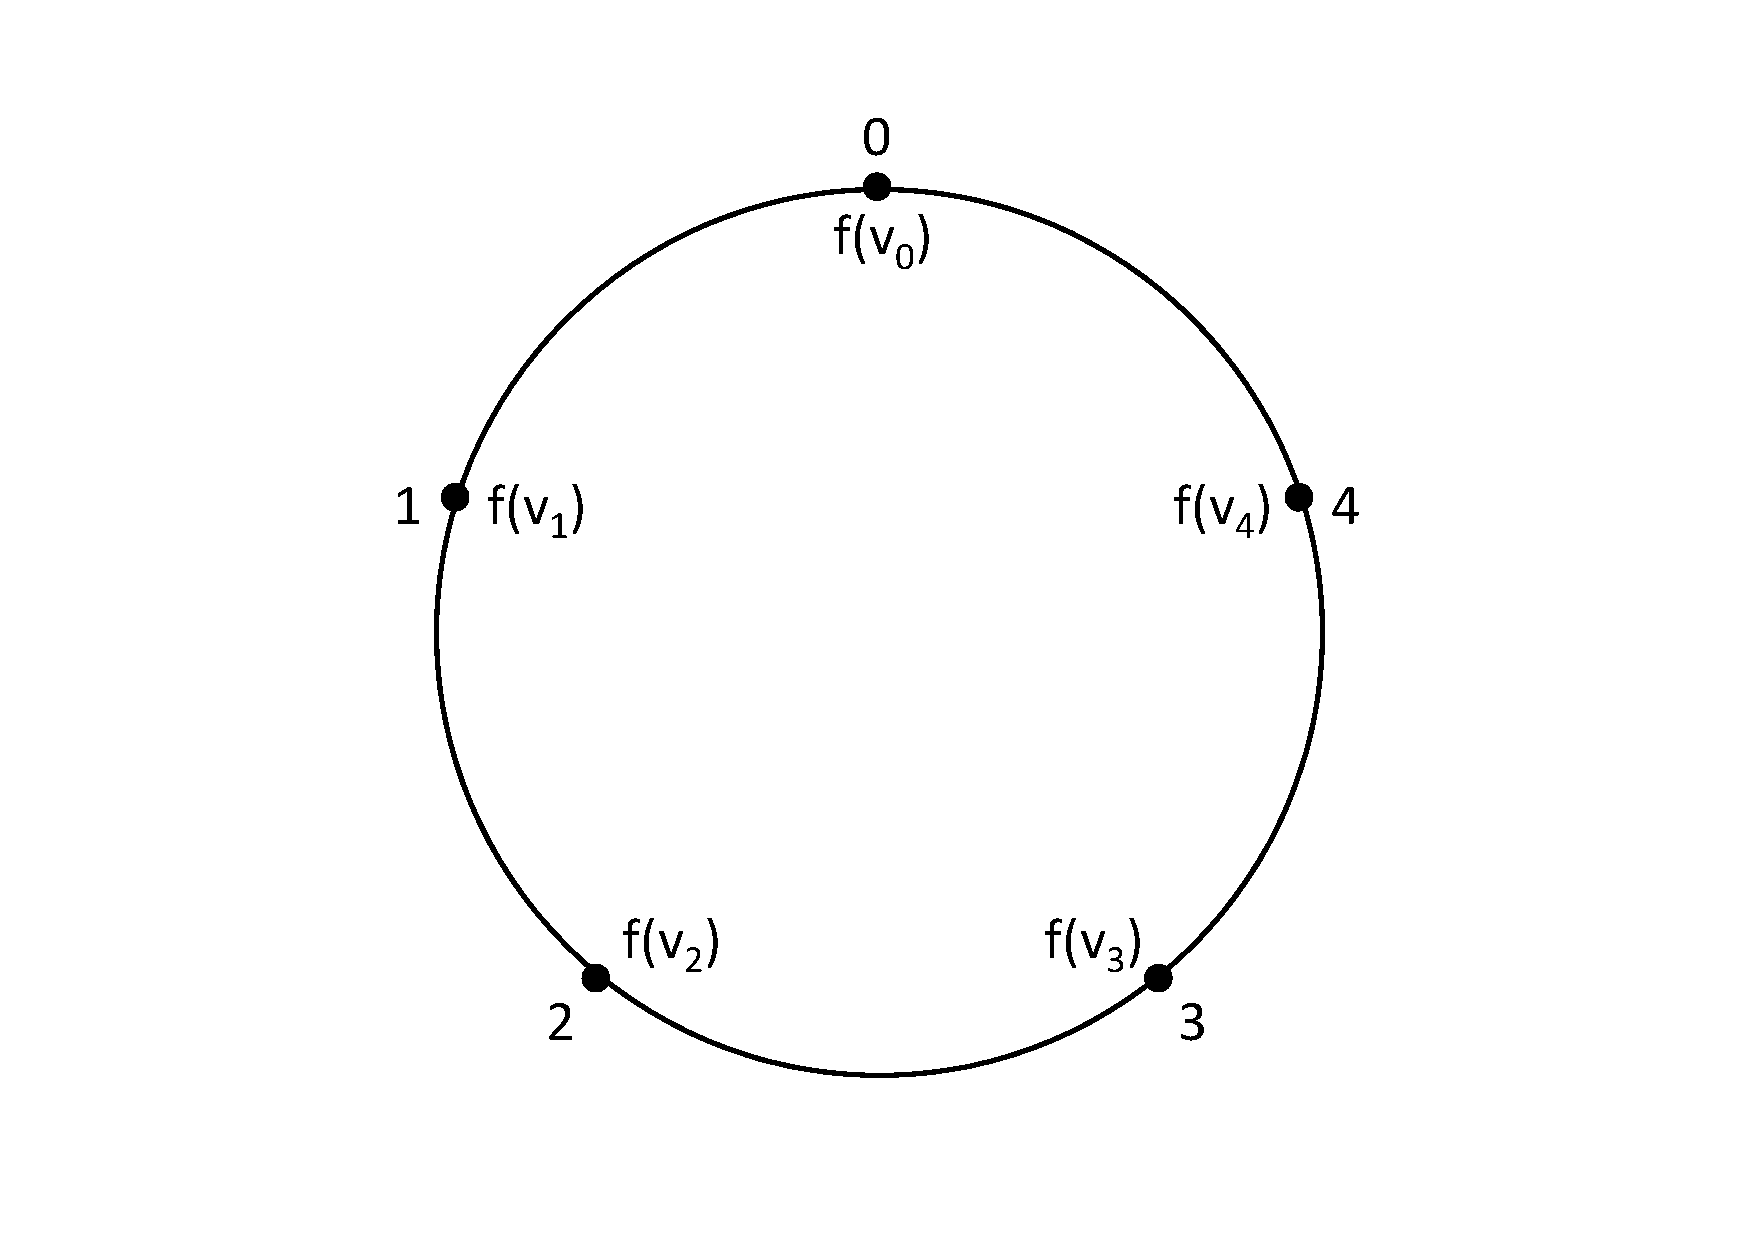
\includegraphics[scale=0.4]{../figures/fig4-1.pdf}
        \vspace{-20pt}
  \caption{Example of cyclic distance}
  \label{cyclic distance}
\end{figure}
\end{example}

\begin{definition}
\label{def:cyclic1}
A cyclic metric $C(p_1, p_2, p_3, \dots)$-labelling of a graph $G$ is a map 
\[
f : V(G) \rightarrow V(C^n) 
\] 
from vertices of $G$ to vertices of a labelled $n$-cycle $C^n$ such that
\[
|\min\{f(u)-f(v), f(v) - f(u)\}| \ge p_{i}\pmod{n}, \text{ if } d_{G}(u, v) = i, \forall i \in [1, \infty) 
\]
where $n \ge 2$ is an integer.  
\end{definition}
\begin{example}
Fixing $C^n$ to be a $5$-cycle; i.e.,  $n = 5$. We can see that Fig. \ref{cyclic labelling} (a) is an $L(2,1,1)$-labelling of $T_{2,2}$, but not a $C(2,1,1)$-labelling, since $|f(u_0) - f(u_2)| = 1 \pmod{6}$ while $d(u_0, u_1) = 1$. Fig. \ref{cyclic labelling} (b) is a $C(2,1,1)$-labelling of $T_{2,2}$. 
\begin{figure}
 \centering
      \vspace{-10pt}
    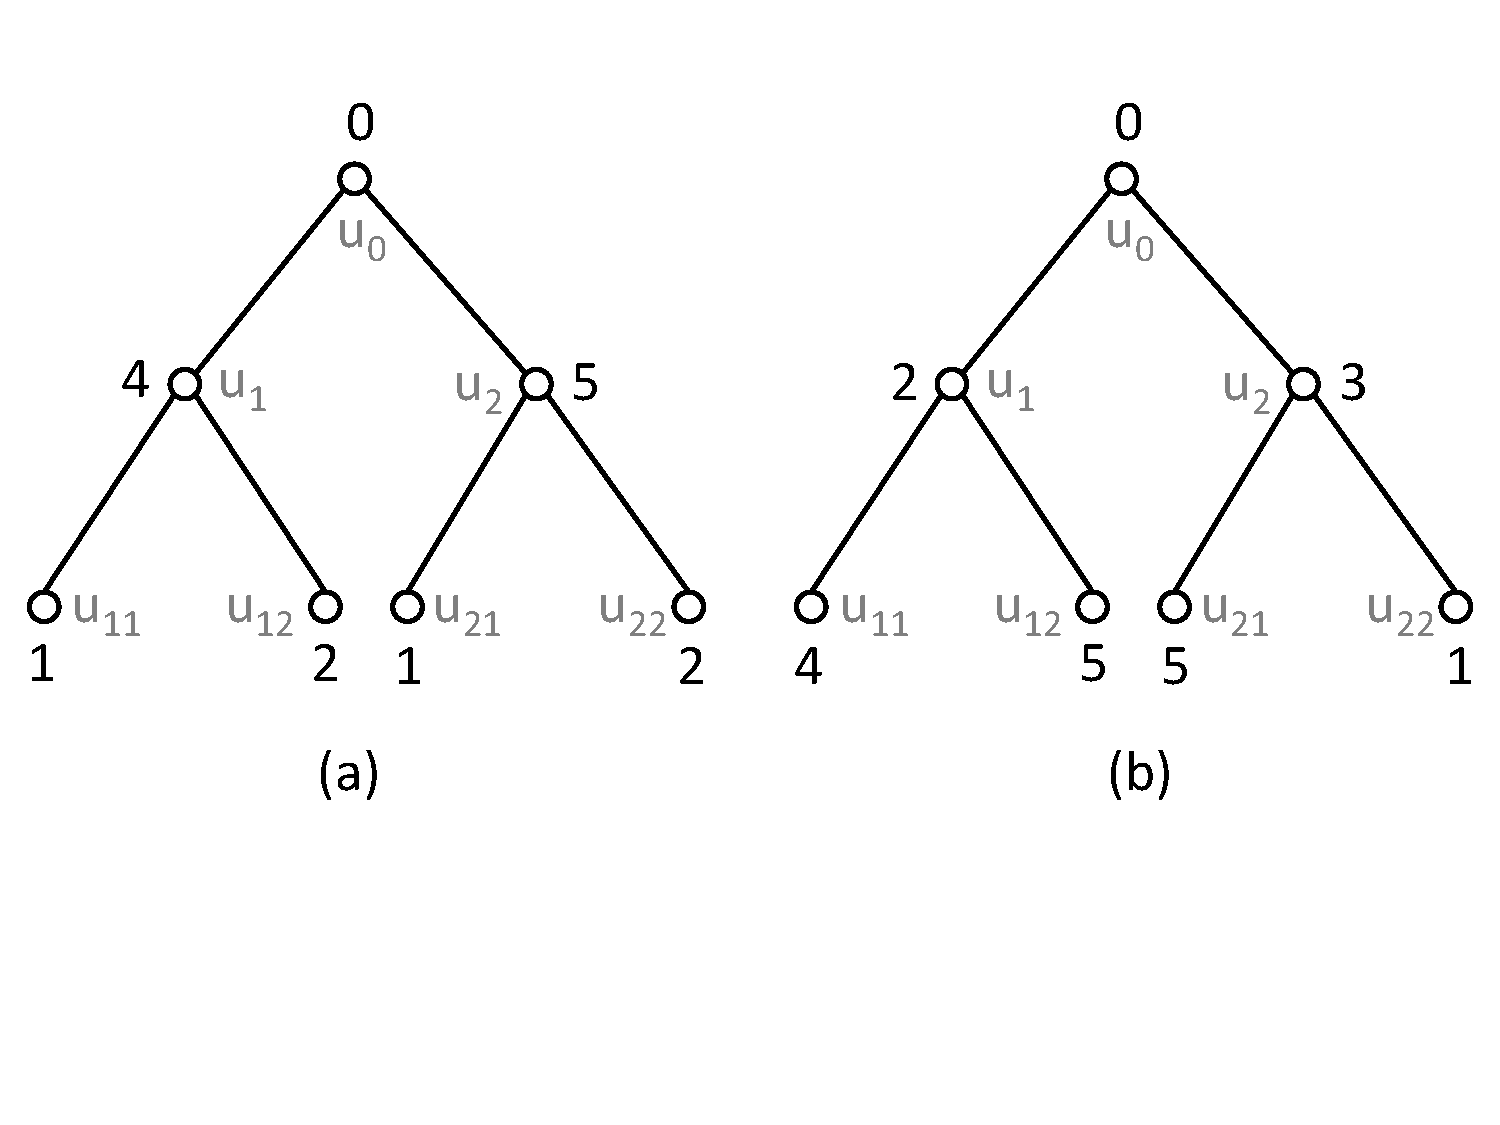
\includegraphics[scale=0.4]{../figures/fig4-2.pdf}
        \vspace{-50pt}
 \caption{Example of $C(2,1,1)$-labelliings of $T_{2,2}$}
  \label{cyclic labelling}
\end{figure}
\end{example}

The aim of cyclic metric labelling problem is to minimise the maximum label used. According to Definition \ref{def:cyclic1}, the objective is to find the smallest integer $n$ for the $n$-cycle that satisfies the above constraint. The $C(p_1, p_2, p_3, \dots)$-labelling is similar to $L(p_1, p_2, p_3, \dots)$-labelling, except this time the function $f$ maps vertices of a graph to vertices of a labelled cycle rather than a path. Of course as there is a unique path between any two vertices on a path, the $L(p_1, p_2, p_3, \dots)$-labelling problem is relatively easier. But the related concepts are still the same as those for linear metric labelling problem.

If a graph $G$ is $C(p_1, p_2, p_3, \dots)$-labelled by a function $f$, then the \emph{span} of the function $f$, $span(f)$, is said to be the difference between the maximum and minimum used labels. Precisely, 
\[
span(f) = \max\{f(u) \mid \forall u \in V(G)\} - \min\{f(u) \mid \forall u \in V(G)\}.
\]
The \emph{minimum span} of $C(p_1, p_2, p_3, \dots)$-labelling of the graph $G$ is then defined as the minimum among all possible $span(f)$. To distinguish it from the minimum span $\lambda_{p_1, p_2, p_3, \dots}(G)$, we use $\t_{p_1, p_2, p_3, \dots}(G)$ to denote the minimum span of $C(p_1, p_2, p_3, \dots)$-labelling of $G$.

%{\bf Technique:}
%Note that when dealing with cyclic metric labelling on complete $m$-ary trees in this chapter, we will not use the technique that we used in the previous chapter. That is, directly finding an optimal labelling on a complete $m$-ary tree $T$, which satisfies the $L(h1,1,)$-labelling constraint. Instead, we will fix a labelled cycle $H$, and try to map vertices of $T$ to vertices of $H$. Since once we can find such a way to map vertices of $T$ to labels of $H$, then we can use the inverse function to map labels of $H$ back to vertices of $T$. 
\begin{corollary}
\label{cor:compare}
For a graph $G$ with $diam(G) \ge 3$, if $\lamhpq(G)$ and $\t_{h,p,q}(G)$ are the minimum spans of the $L(h,p,q)$ and $C(h,p,q)$-labelling of $G$ respectively, then 
\begin{align*}
\lambda_{h,p,q}(G) \le \t_{h,p,q}(G).
\end{align*} 
\end{corollary}

\begin{proof}
This corollary follows from the definition of cyclic metric labelling naturally. If we have the graph $G$ is both $\chpq$ and $\lhpq$-labelled with the minimum spans $\thpq(G) < \lambda_{h,p,q}(G)$, then by deleting the edge between $0$ and $\t_{h,p,q}(G)$ on the labelled $n$-cycle $C^n$ we get another function, which $\lhpq$-labels $G$ with a smaller minimum span. This contradicts the assumption that $\lambda_{h,p,q}(T)$ is the minimum span.  
\end{proof}
\qed

When mapping vertices of a graph to a labelled path, we always start from the label $0$ as we aim for achieving the smallest maximum label. However, when mapping them to a labelled cycle, there is no fixed starting point, as there is no difference between starting from label $0$ or $1$. The next definition defines an equivalence relation between two $C(h,p,q)$-labellings. 

\begin{definition}
\label{def:equi}
Let 
\[
f_1 : V(G) \rightarrow V(C_1^n)
\]
and
\[
f_2: V(G) \rightarrow V(C_2^n)
\]
be two different $C(h,p,q)$-labellings of a graph $G$. We say the function $f_{1}$ is equivalent to $f_{2}$ if the two labelled $n$-cycles are identical and $f_1(V(G)) = R \circ f_2(V(G))$, where $R$ is a rotation of $C^n$. 

Precisely, if $C_1^n = C_2^n$ and $f_1(V(G)) = f_2(V(G)) +r \pmod n$, where $r \in [0,n-1]$ is an integer, then the function $f_1$ is said to be equivalent to $f_2$, denoted by   $f_{1} \sim f_{2}$. 
\end{definition}

\begin{example} 
Let $f_1$ and $f_2$ be two different $C(2,1,1)$-labellings of the complete $2$-ary tree $T_{2,2}$. (Fig. \ref{fig equivalent}) It is obvious that the labelled $5$-cycles are identical. Also, $f_1(V(T_{2,2})) +2= f_2(V(T_{2,2})) \pmod 6$. Hence, the two $C(2,1,1)$-labellings are equivalent. 
\begin{figure}
  \centering
    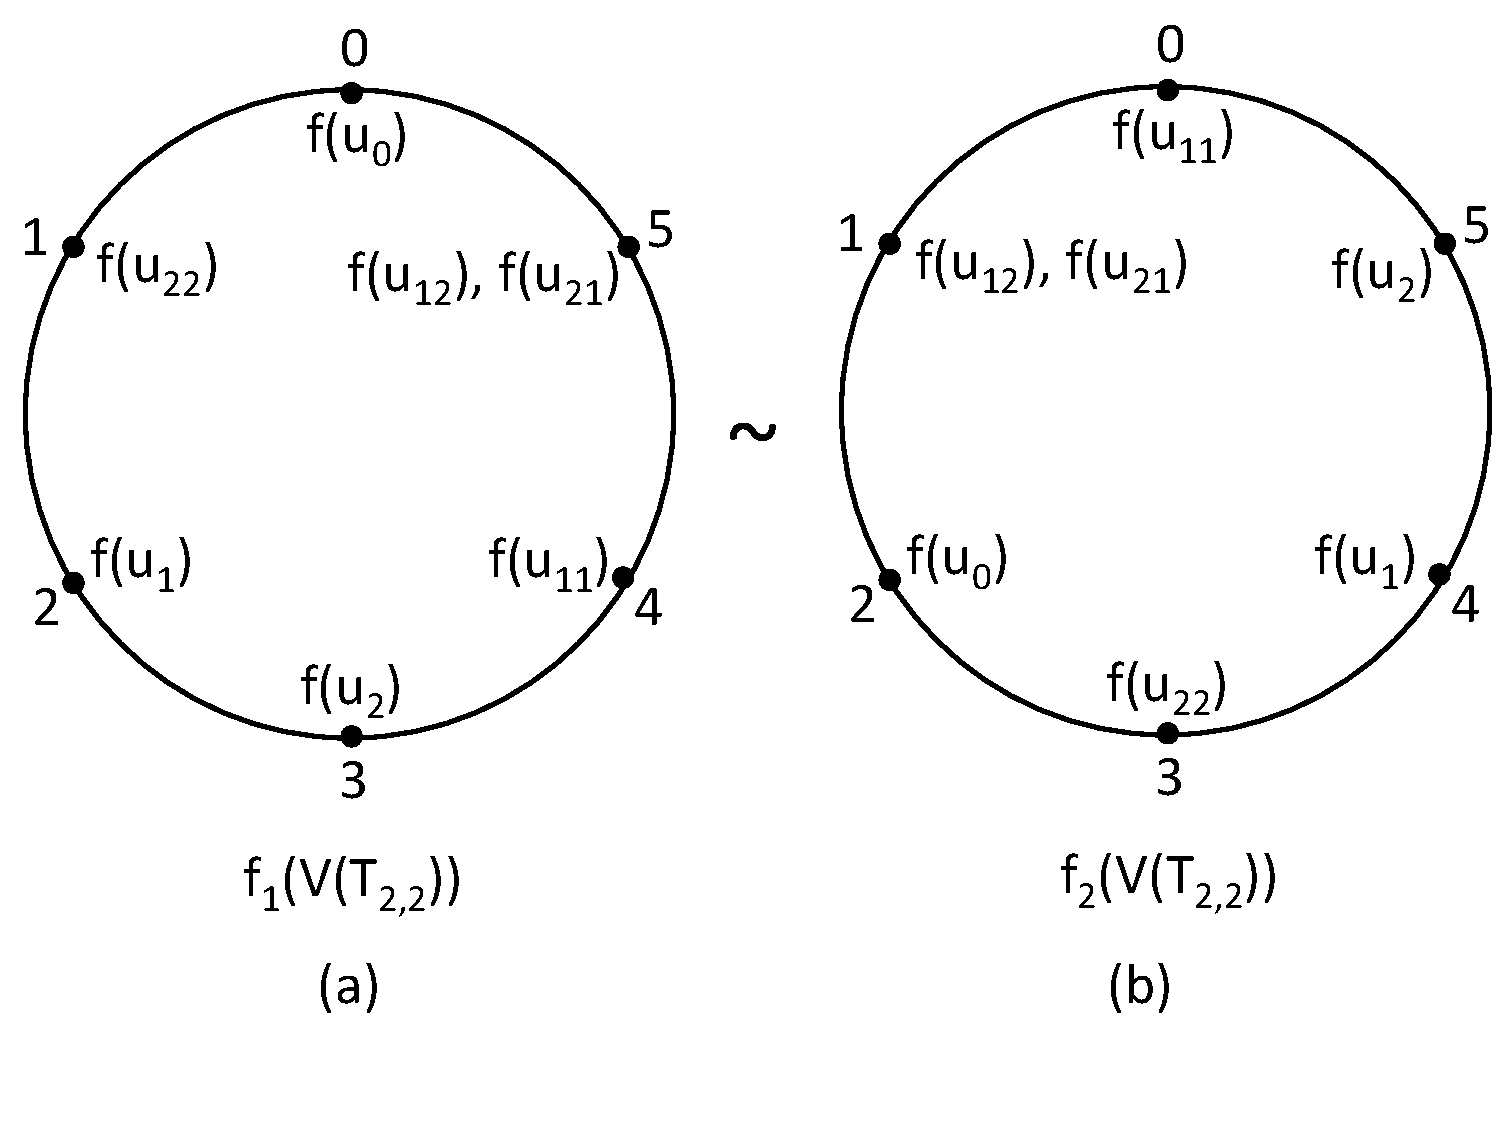
\includegraphics[scale=0.4]{../figures/fig4-3.pdf} 
    \vspace{-10pt}
\caption{Equivalent relation between two $C(h,1,1)$-labellings of a $T_{2,2}$}
\label{fig equivalent}
\end{figure} 
\end{example}

\begin{remark}
\label{rmk:fix0}
From now on, we assume without loss of generality that if $f$ is a $C(h,p,q)$-labelling of a tree $T$, then the root of $T$ is always assigned the label $0$. Since if it does not, then we can rotate $C^n$ to make sure the root of $T$ obtaining $0$. The rotation is well-defined according to Definition \ref{def:equi}.
\end{remark}


%\begin{proposition}
%Let $T$ and $H$ be defined as above. Let $f_{1}$ and $f_{2}$ be two $C_{h,1,1}$-labelling functions, which takes vertices $u$ and $v$ as the first vertex maps to the cycle $H$ respectively. Then, we have $f_{1} \sim f_{2}$.  
%\end{proposition}






%%%%%%%%%%%%%%%%%%%%%%%%%%%%%%%%%%%%
\section{Known results for cyclic metric labelling problem} 
As the cyclic metric labelling problem is not as widely studied as the linear metric labelling problem, we will only review this problem for outerplanar graphs. 
\subsection{Outerplanar graphs}

In section \ref{linear outerplanar}, we mentioned that \cite{bodlaender04} conjectured the minimum span of the $L(2,1)$-labelling of outerplanar graphs $G$ is bounded above by $\Delta+2$. Motivated by this conjecture, \cite{liu05} proved results for cyclic metric labelling of outerplanar graphs $G$ under distance two constraints. In particular, they proved \citeauthor{bodlaender04}'s conjecture to be true, but only for outerplanar graphs with large maximum degree. The authors first proved a connection between the minimum span of the $L(2,1)$ and $C(2,1)$-labelling of outerplanar graphs; i.e.,  
\begin{align}
\label{relation1}
\lambda_{2,1}(G) \le \t_{2,1}(G) \le \lambda_{2,1}(G) +2.
\end{align}
Then they proved that for any outerplanar graph $G$ with the maximum degree $\Delta(G) \ge 15$, the minimum span of $C(2,1)$-labelling is $\t_{2,1}(G) = \Delta+3$. By this result and \eqref{relation1}, \citeauthor{bodlaender04}'s conjecture is proved, but only for $G$ with large maximum degree. They also proved the following.
\begin{theorem}
For any outerplanar graph $G$, the minimum span  $\t_{2,1}(G) \le \Delta+7$. Moreover, if $G$ is triangulated then $\t_{2,1}(G) \le \Delta +5$. 
\end{theorem}
\begin{theorem}
If $G$ is an outerplanar graph and $\Delta \ge 11$ then $\t_{2,1}(G) \le \Delta + 4$. 
\end{theorem}

For outerplanar graph $G$ with small maximum degree. ($\Delta \in [2,5]$) \cite{liu05} proved that the minimum span $\t_{2,1}(G) = \Delta+ 4$.

In the next section, we will present to the reader our results of $C(h,1,1)$-labelling of complete $m$-ary trees. 

%%%%%%%%%%%%%%%%%%%%%%%%
\section{The $C(h,1,1)$-labelling problem}
\label{sec:cyc}
Our results are separated into two parts based on the height of a complete $m$-ary tree. The first part deals with the problem of complete $m$-ary trees $\tmk$ with height $k=2$, while the second part deals with the case when $k \ge 3$. 


%%%%%%%%%%%%%%%%%%%%%%%%%%%%%%%%%%%%

\subsection{Complete $m$-ary tree with height $2$}
Recall that we only deal with the $\lhpq$ and $\chpq$-labelling problems for $h \ge 2$. This assumption is used throughout this thesis.
\begin{remark}
For a complete $m$-ary tree $\tmk$ with $k \ge 2$, the $C(1,1,1)$-labelling problem is the same as the $L(1,1,1)$-labelling problem. In other words, we have $\t_{1,1,1}(\tmk) = \lambda_{1,1,1}(\tmk)$, for $k \ge 2$. 
\end{remark}

The next theorem is the major result for the $C(h,1,1)$-labelling problem of $\tm2$. It also indicates the connection of the minimum spans of these two labellings. 
\begin{theorem}
\label{thm:ck2}
For a complete $m$-ary tree $\tm2$, the minimum span of the $C(h,1,1)$-labelling is  
\begin{align}
\label{ck2}
\t_{h,1,1}(\tm2) &= \max\{\lamh11(\tm2), \lamh11(\tm2)+h-m\}\\
\label{ck22}
&= \max\{2m+h-1, 2h+m-1\}.
\end{align}
\end{theorem}

\eqref{ck22} is a consequence of \eqref{ck2} provided Theorem \ref{thm:h11} is known. The value $2m+h-1$ is achieved for $h\le m$, while $2h+m-1$ is achieved for $h \ge m$. 
\\
\begin{proof} The first step is to prove the minimum span $\t_{h,1,1}(\tm2) \ge  \max\{2m+h-1, 2h+m-1\}$. By Corollary \ref{cor:compare}, we have $\lambda_{h,1,1}(\tm2) \le \t_{h,1,1}(\tm2)$. It follows that $\t_{h,1,1}(T) \ge 2m+h-1$. 

To complete the first step, we need to show the minimum span also satisfies $\t_{h,1,1}(\tm2) \ge 2h+m-1$. This can be proved by contradiction. Assume $\th11(\tm2) \le 2h+m-2$. Then there exists a $C(h,1,1)$-labelling 
\[
f:V(\tm2) \rightarrow V(C^n)
\]
from vertices of height $2$ complete $m$-ary trees to a labelled $n$-cycle, such that $span(f) = 2h+m-2$. By Remark \ref{rmk:fix0}, the root $u_0$ bears the label $0$. As $u_i \in C(u_0)$, for the function $f$ to be a $C(h,1,1)$-labelling of $\tm2$, we must have $f(C(u_0))=\{f(u_{i}) \mid i \in [1,m]\} \subseteq [h, h+m-1]$. Since the cardinality of the set $[h, h+m-1]$ is $m$, it follows $\{f(u_{i}) \mid i \in [1,m]\} = [h, h+m-1]$. Without loss of generality, assume $f(u_i) = h+i-1$. Then we have $f(u_1) = h$ and $f(C(u_1)) \subseteq [2h, 2h+m-2]$, see Fig. \ref{4.3}. There are only $m-1$ labels in the set $[2h, 2h+m-2]$, while the cardinality of $C(u_1)$ is $m$ and each vertex requires a distinctive label. Hence, the assumption $span(f) = 2h+m-2$ is not sufficient to $C(h,1,1)$-label $\tm2$. Therefore, we must have $\t_{h,1,1}(\tm2) \ge 2h+m-1$ when $h \ge m$.
\begin{figure}
  \centering
     \vspace{-0pt}
    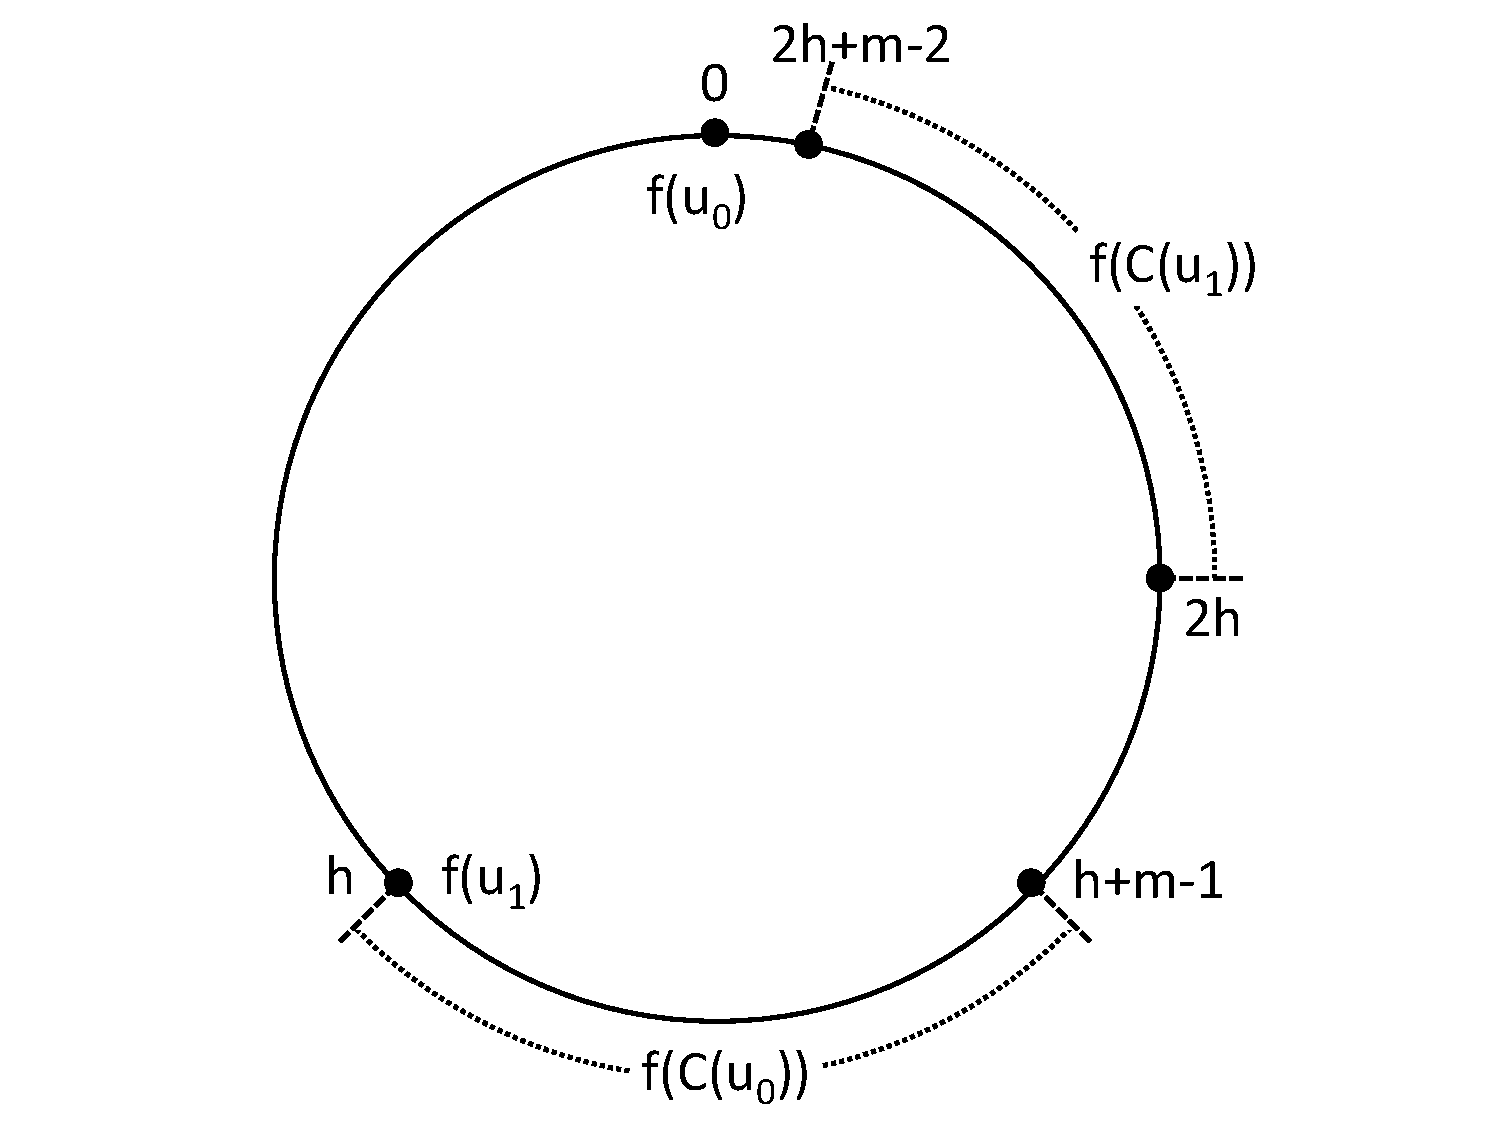
\includegraphics[scale=0.35]{../figures/fig4-4.pdf}
    \vspace{-0pt}
\caption{$span(f) = 2h+m-2$ is not sufficient to $C(h,1,1)$-label $\tm2$}
\label{4.3}
\end{figure}

So far we have proved that $\t_{h,1,1}(\tm2) \ge  \max\{2m+h-1, 2h+m-1\}$. It remains to show that $\t_{h,1,1}(T) \le \max\{2m+h-1, 2h+m-1\}$. If we can find a function $f : V(\tm2) \rightarrow V(C^n)$ with $span(f) = \max\{2m+h-1, 2h+m-1\}$, then we are done. 

Notice that the function $f$ varies for different values of $h$ and $m$. If $h \le m$, then $f$ labels $\tm2$ as follows: 
\begin{enumerate}[(1)]
\item $f(u_0) = 0$;
\item $\{f(u_i) \mid i \in [1,m]\} = [h,h+m-1]$ such that $f(u_i) = h+i-1$;
\item If $i \in [1, m-h+1]$, then $f(C(u_i)) = [h+m, 2m+h-1]$; \\if $i \in [m-h+2, m]$, then $f(C(u_i)) = [2h+i-1, m+2h+i-1] \setminus \{0\}  \pmod {2m+h}$.
\end{enumerate}
On the other hand, if $h \ge m$, then the function $f$ is defined as follows: 
\begin{enumerate}[(1)]
\item $f(u_0) = 0$;
\item $\{f(u_i) \mid i \in [1,m]\} = [h,h+m-1]$ such that $f(u_i) = h+i-1$;
\item $f(C(u_i)) = [2h+i-1, 2h+m+i-1] \setminus \{0\} \pmod {2h+m}$.
\end{enumerate}

It is not hard to check that the function $f$ defined above indeed is a $C(h,1,1)$-labelling of $\tm2$ with $span(f) = \max\{2m+h-1, 2h+m-1\}$. Moreover, the two cases of $f$ are identical when $h = m$. 
\end{proof}
\qed


%%%%%%%%%%%%%%%%%%%%%%
\subsection{Complete $m$-ary trees with height no less than $3$}
\begin{theorem}
\label{thm:ck3}
For a complete $m$-ary tree $\tmk$ with height $k \ge 3$, the minimum span of the $C(h,1,1)$-labelling is \begin{align}
\t_{h,1,1}(T) & = \max\{\lambda_{h,1,1}(\tmk), \lambda_{h,1,1}(\tmk)+h-m-1\} \\
\label{eq:bd1}
&= \max\{2m+h, 2h+m-1\}.
\end{align}
\end{theorem}

Similarly, $\lambda_{h,1,1}(\tmk)$ achieves $2m+h$ when $h \le m+1$, $2h+m-1$ when $h \ge m+1$. 

\begin{proof}
The same method is used to prove this theorem. That is, by showing the lower and upper bounds of the minimum span $\t_{h,1,1}(T)$ are identical.   

Corollary \ref{cor:compare} implies $\t_{h,1,1}(\tmk) \ge \lambda_{h,1,1}(\tmk) = 2m+h$ for $k \ge 3$. We also need to show $\t_{h,1,1}(\tmk) \ge 2h+m-1$. According to Theorem \ref{thm:ck2}, the minimum span $\t_{h,1,1}(\tm2) = 2h+m-1$ for $h \ge m$. Hence, it is obvious that the minimum span will be no less than $2h+m-1$ for larger complete $m$-ary trees $\tmk$ with $k \ge 3$. Precisely, $\t_{h,1,1}(\tmk) \ge 2h+m-1$ for $k \ge 3$.   

The trick of the proof is to find a function $$f:V(\tmk) \rightarrow V(C^n)$$ such that a complete $m$-ary tree $\tmk$ with $k \ge 3$ is $C(h,1,1)$-labelled by $f$ with
\[
span(f) =  \max\{2m+h, 2h+m-1\}.
\]
Lemma \ref{lem:consecutive} below proves the existence of such a function. 
\end{proof}
\qed

We are dealing with all complete $m$-ary trees $\tmk$ with $k \ge 3$. Hence, the height of such a tree could be infinite. The objective of this problem is to map vertices of $\tmk$ to vertices on a labelled $n$-cycle with $n$ as small as possible. 

For the cyclic metric, when mapping vertices of $\tmk$ to vertices on a cycle, the mapping can go around the cycle again and again. Hence the degree of difficulty involved in establishing a pattern is increase.  

Nevertheless, the essential observation is that the neighbours of every internal vertex can be mapped to a consecutive set of vertices on $C^n$. The following lemma states this observation explicitly, but in a slightly different family of trees

In Definition \ref{neighbour}, we defined the neighbours of a vertex $u \in V(G)$ in graph $G$ to be the set of vertices adjacent to $u$; i.e.,  $N(u) := \{v \in V(G) \mid d(u,v) = 1\}$. We define another notation $\overline{N(u)} :=\{u\} \cup N(u)$.

\begin{lemma}
\label{lem:consecutive}
Let $\tilde{T}$ be a complete $m$-ary tree with an extra edge attached to the root of it; i.e.,  $\tilde{T} := \tmk +\{u_0v\}$, where $v$ is the root $\tmk$. Then, there is a $C(h,1,1)$-labelling $f: V(\tilde{T}) \rightarrow V(C^n)$ such that 
\begin{enumerate}[(1)] 
\item $span(f) = \max\{2m+h, 2h+m-1\}$;
\item for any vertex $u \in V(\tilde{T})$ with $d(u) = m+1$, its neighbours $N(u)$ can be labelled consecutively by the map $f$ for all values of $h$ and $m$.   
\end{enumerate}
\end{lemma}   

The way we construct $\tilde{T}$ means that every complete $m$-ary tree $\tmk$ is covered by a $\tilde{T}$. Accordingly, if the lemma holds for $\tilde{T}$, then it also holds for $\tmk$. 
\\
\begin{proof}
The first step is to use induction to show $(2)$, provided $\max\{V(C^n)\} = \t_{h,1,1}(\tilde{T})$. The following are the two inductive steps: 
\begin{enumerate}[(i)]
\item for the root $u_0$ of $\tilde{T}$, $f(N(u_0))$ is a consecutive set of labels.
\item for any vertex $u_{0\dots jk} \in V(\tilde{T})$ with $d(u_{0\dots jk}) = m+1$, if $u_{0\dots jk}$ and $N(u_{0\dots jk})$ have been labelled, and $f(N(u_{0\dots jk}))$ is assigned a consecutive label set, then $f(N(u_{0\dots jkl}))$ can also be assigned a consecutive label set, for any vertex $u_{0\dots jkl} \in C(u_{0\dots jk})$ with $d(u_{0\dots jkl}) = m+1$. 
\end{enumerate} 

Without loss of generality, assume label $u_0$ and its neighbours $N(u_0)$ first. In this case, $f(N(u_0))$  is a consecutive part on $C^n$. Then step (i) is trivial. 

To prove step (ii), we note that if the function $f$ is a $C(h,1,1)$-labelling of $\tilde{T}$, then it needs to satisfy the following condition when labelling $C(u_{0\dots jkl})$:  
\begin{align}
\label{condition1}
&f(C(u_{0\dots jkl})) \subseteq V(C^n) \setminus (S \cup W)
\end{align}  
where 
\begin{align*}
S &:= f(\overline{N(u_{0\dots jk})}) \\
W &:= [f(u_{0\dots jkl}) - (h-1), f(u_{0\dots jkl}) + (h-1)].
\end{align*}

The cardinality $|S| = m+2$ by definition. Moreover, by assumption in (ii) we have $f(N(u_{0\dots jk}))$ is consecutive. Thus the set $S$ consists of one consecutive segment and one single label with a separation at least $h$. The way $W$ is defined ensures that it is consecutive with cardinality $|W| = 2h-1$. Moreover, $S \cap W \neq \emptyset$, since $u_{0\dots jkl} \in N(u_{0\dots jk})$. This implies $Q:=f(N(u_{0 \dots jk})) \cup W$ is still a consecutive segment of larger cardinality. Notice that $f(u_{0\dots jk}) \not\in Q$, as it has separation at least $h$ with $f(N(u_{0\dots jk}))$. But it can be adjacent $Q$. Hence $S\cup W$ is either a consecutive set or a consecutive set union single label. Equivalently, $V(C^n) \setminus (S \cup W)$ consists of either one consecutive set or two consecutive sets separated by $f(u_{0\dots jk}) \cup Q$ (Fig. \ref{lemma ex 1}, Fig. \ref{lemma ex 11}).

\begin{figure}
 \centering
     \vspace{-0pt}
    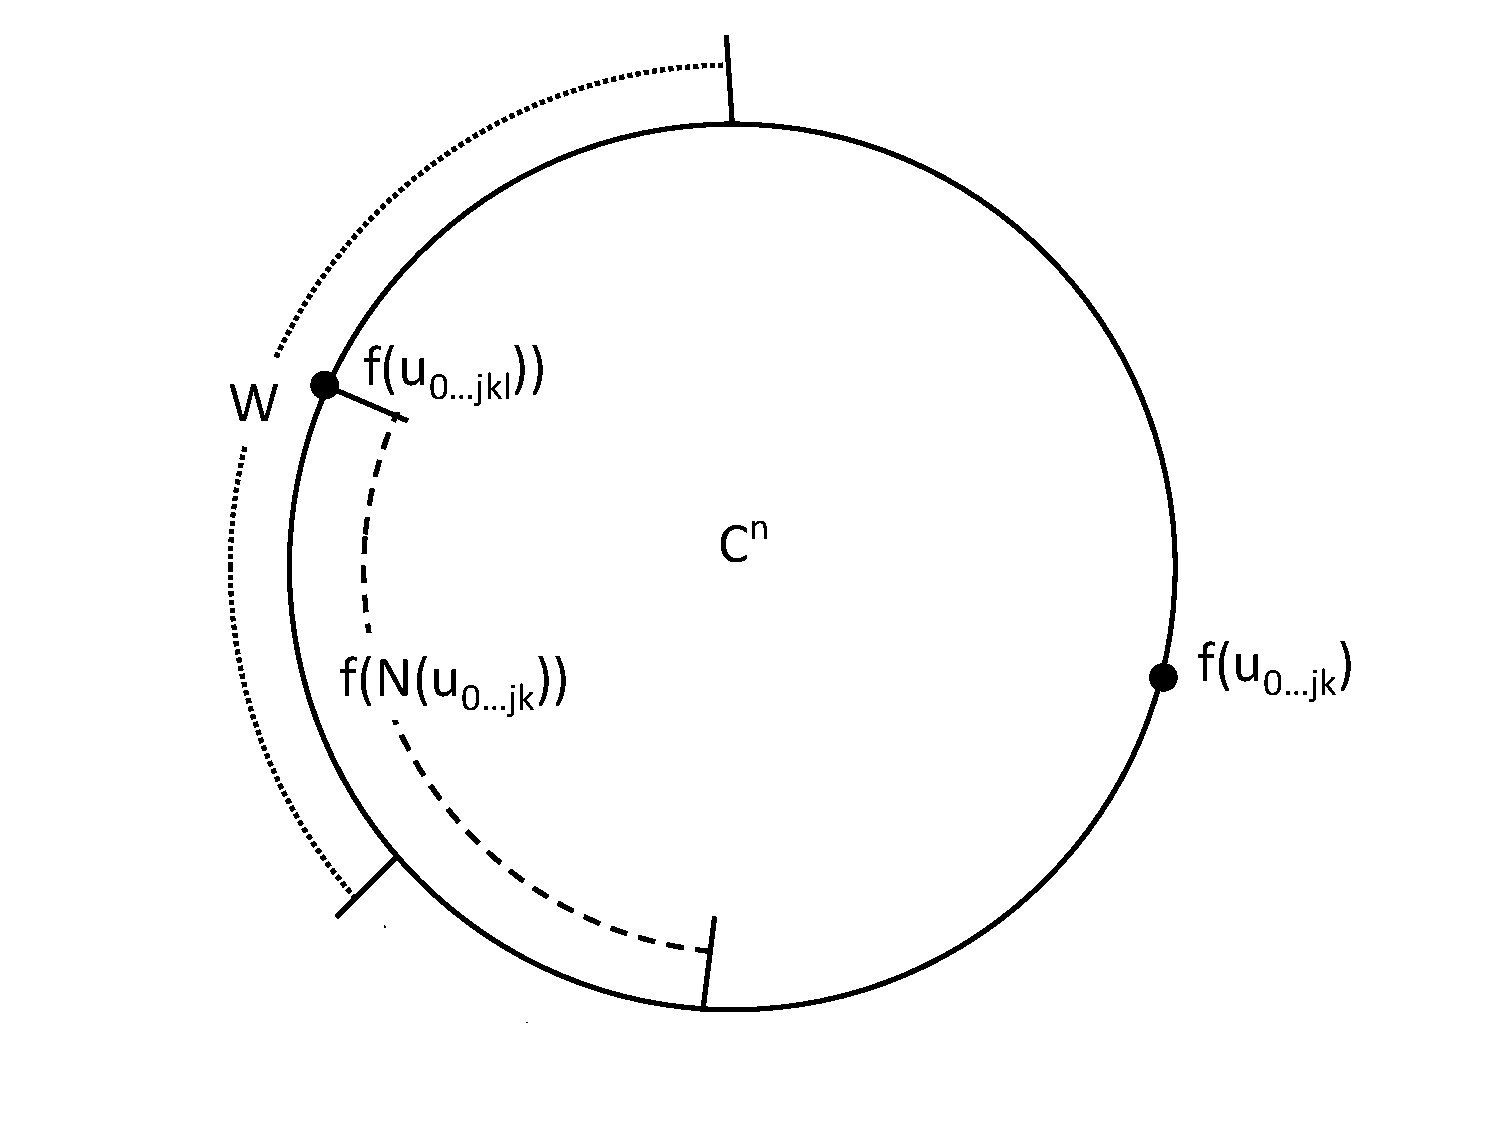
\includegraphics[scale=0.45]{../figures/fig4-5-a.pdf}
   \vspace{-0pt}
\caption{Two consecutive sets for $C(u_{0\dots jkl})$} 
\label{lemma ex 1}
\end{figure}

\begin{figure}
 \centering
     \vspace{-0pt}
    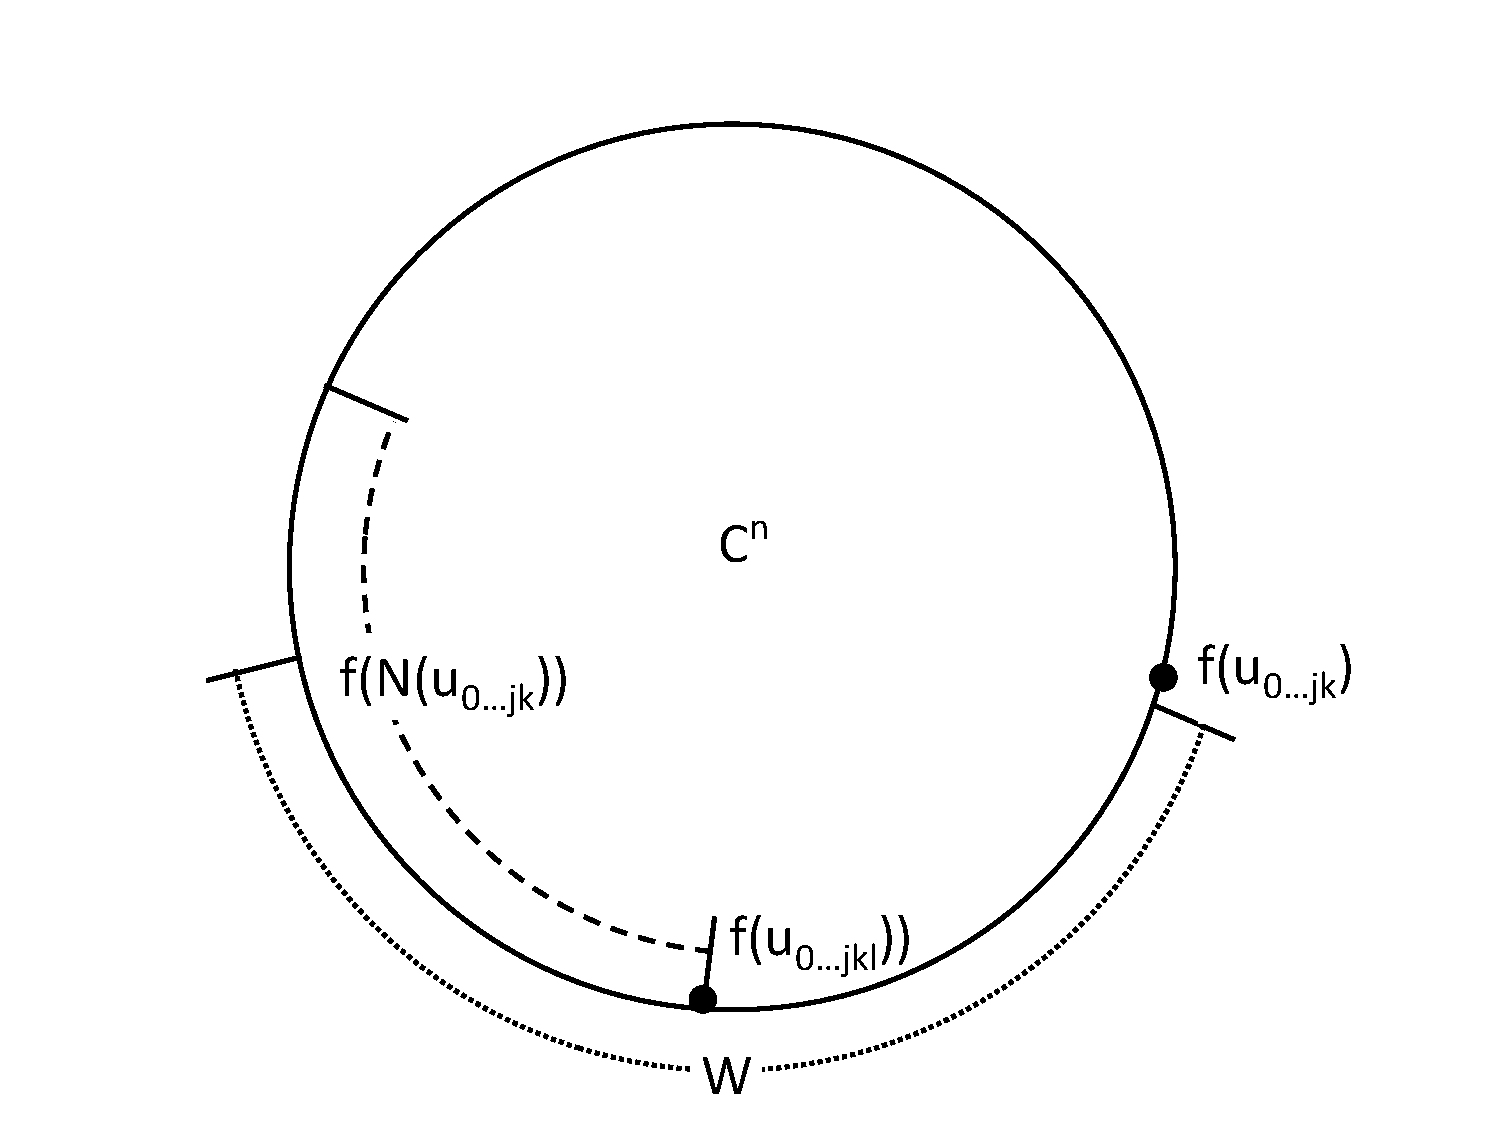
\includegraphics[scale=0.45]{../figures/fig4-5-b.pdf}
   \vspace{-0pt}
\caption{One consecutive set for $C(u_{0\dots jkl})$} 
\label{lemma ex 11}
\end{figure}
 

Use $(S \cup W)^c$ to denote $V(C^n) \setminus (S \cup W)$ now. Since $u_{0\dots jk} \in N(u_{0\dots jkl})$, then 
\begin{align}
\label{equ:condition2}
f(N(u_{0\dots jkl})) \subseteq (S \cup W)^c \cup \{f(u_{0\dots jk})\}.
\end{align}

\eqref{equ:condition2} implies that in either case $f(N(u_{0\dots jkl}))$ is a consecutive set. Thus (ii) is proved.

In fact, it is not hard to see that the cardinality of the set $Q$ is dependent upon the position of $u_{0\dots jkl}$ in $N(u_{0\dots jk})$. In particular, it obtains the largest cardinality when $u_{0\dots jkl}$ is one of the end points of $N(u_{0\dots jk})$. Equivalently, $S \cup W$ reaches its maximum size when the intersection $S\cap W$ has the smallest cardinality, as $|S \cup W| = |S| + |W| - |S \cap W|$. Thus to compute the cardinality of $S\cup W$, we consider the following two cases. 

If $h < m$, then $\min\{|S \cap W|\} = h$. This occurs when $u_{0\dots jkl}$ is one of the end points of $N(u_{0\dots jk})$. Thus we have 
\begin{align*}
|S \cup W| &= |S| + |W| - |S \cap W| \\
& \le |S| + |W| - \min\{|S \cup W|\} \\
& = (m+2) + (2h-1) - h\\
&= m+h+1.
\end{align*}

Since $\tau_{h,1,1}(\tilde{T}) = 2m+h$ when $h < m$, then $|V(C^n)| = 2m+h+1$. Thus we have 
\begin{align*}
|V(C^n) \setminus (S \cup W)| &= |V(C^n)| - |S\cup W|\\
& \ge (2m+h+1) - (m+h+1) \\
&= m.
\end{align*}
This shows that there are just enough labels for the function $f$ to $C(h,1,1)$-label $C(u_{0\dots jkl})$, as $|C(u_{0\dots jkl})| = m$. 

If $h \ge m$, the situation is easier, because the set $f(N(u_{0\dots jk})) \subsetneq W$ is contained in $W$ as a subset, no matter where $u_{0\dots jkl}$ is located in the set $N(u_{0\dots jk})$ (Fig. \ref{lemma ex 2}). Hence, $|S \cup W| = |W| +1= 2h$. This implies 
\begin{align*}
 |V(C^n) \setminus (S \cup W)| &=
 \begin{cases}
 (2m+h+1) -2h & \text{ if } h =m,\\
 (2h+m)-2h & \text{ if } h \ge m+1.
 \end{cases}\\
&=  \begin{cases}
   m+1 & \text{if } h = m,\\
   m       & \text{if } h \ge  m+1.
  \end{cases}
\end{align*}
This also shows there are enough labels for the function $f$ to $C(h,1,1)$-label $C(u_{0\dots jkl})$. This completes the proof.  
\end{proof}
\qed
\begin{figure}
 \centering
     \vspace{-10pt}
    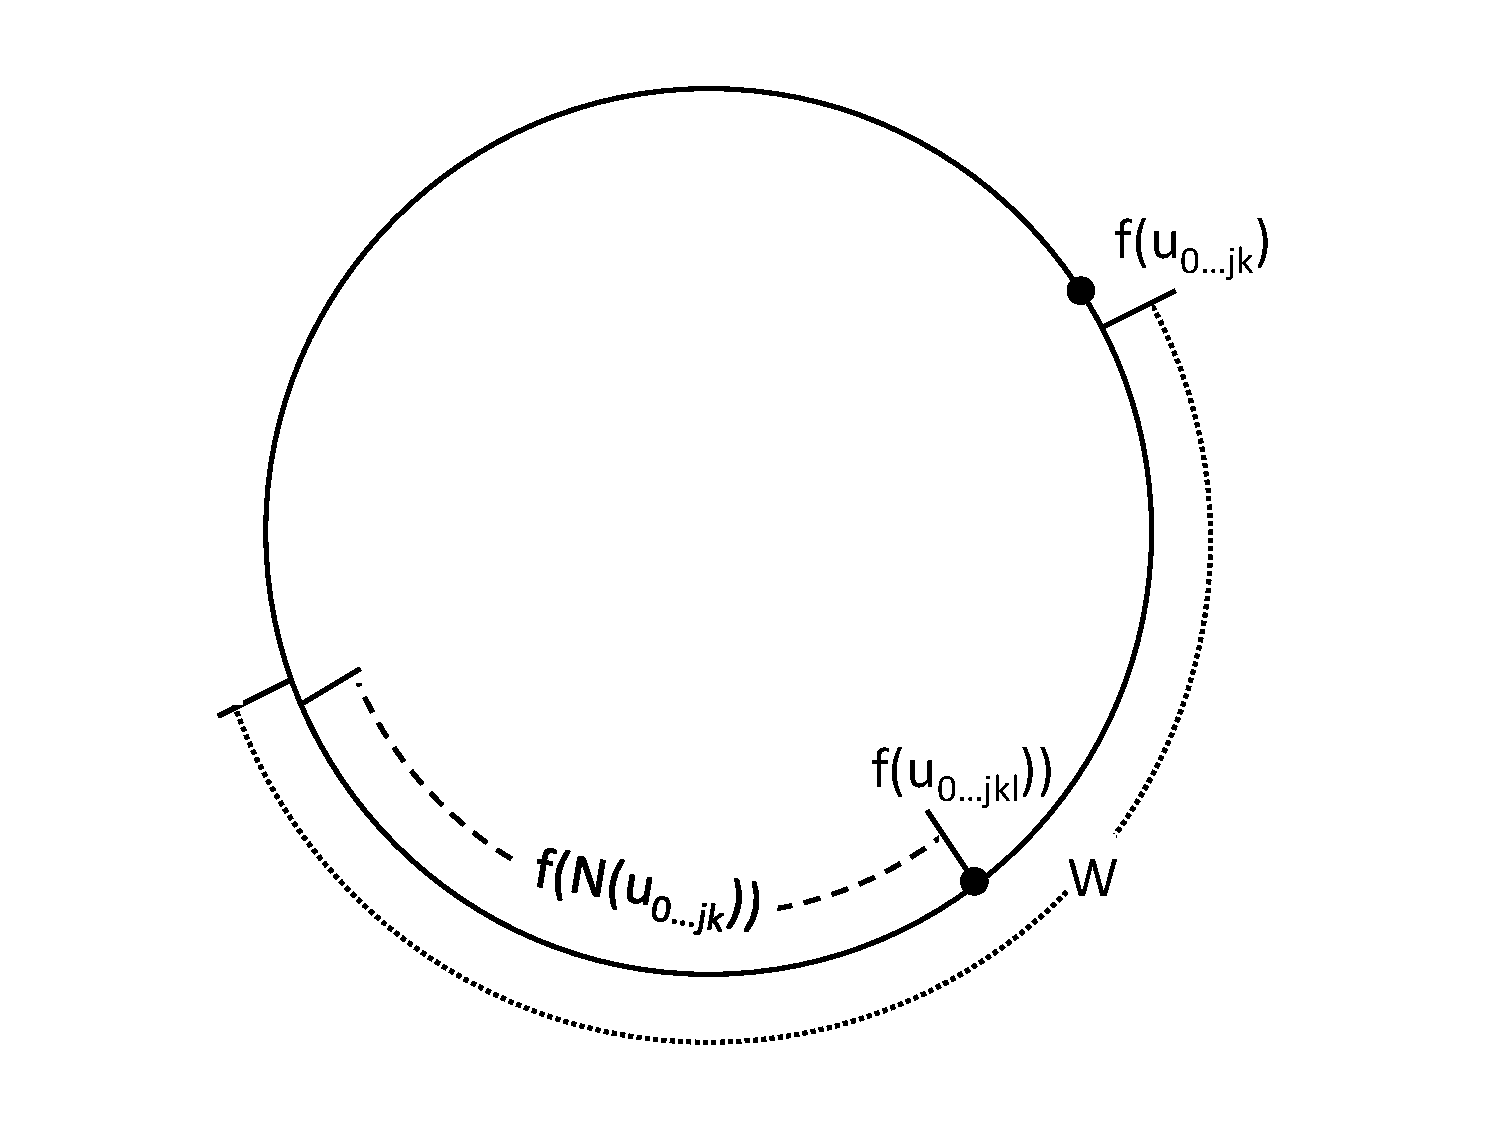
\includegraphics[scale=0.4]{../figures/fig4-7.pdf}
    \vspace{-0pt}
\caption{Special case when $f(N(u_{0\dots jk})) \subsetneq W$} 
\label{lemma ex 2}
\end{figure}


If we apply this lemma to complete $m$-ary trees $\tmk$ with height $k \ge 3$, then obviously it ensures the existence of a function $f$, which $C(h,1,1)$-labels $\tmk$ with the minimum span $\t_{h,1,1}(\tmk) = \max\{2m+h, 2h+m-1\}$ for $k \ge 3$. Thus Theorem \ref{thm:ck3} is proved. 

\begin{remark}
\label{howtolabel}
Lemma \ref{lem:consecutive} in fact gives an almost explicit way of how to label vertices of a complete $m$-ary tree $\tmk$ for $k \ge 3$. In the proof we see that \eqref{condition1} gives an exact label set for $C(u_{0\dots jkl})$ when $h<m$, while it provides $1$ extra label when $h \ge m+1$ and $2$ extra labels when $h=m$. 
\end{remark}

In this section, we solved the $C(h,1,1)$-labelling problem of complete $m$-ary trees. We proved that the minimum span $\t_{h,1,1}(\tm2)$ and $\t_{h,1,1}(\tmk)$ for $k \ge 3$ can be solved exactly, but dependent upon the values of $h$ and $m$. In the next section, we are aiming for generalising these results to $\chpq$-labelling problems of complete $m$-ary trees. 

%%%%%%%%%%%%%%%%%%%%%%%%%%%%%%%%%%%%
\section{The $C(h,p, q)$-labelling problem}

In this section, we extend our previous study of the cyclic metric labelling problem to a more general version, the $C(h,p,q)$-labelling problem, where $h \ge p \ge q \ge 1$. The set of trees we will deal with in this section is still the set of complete $m$-ary trees. 


%%%%%%%%%%%%%%%%%%%%%%%%%%%%%%%%%%%%


\subsection{Complete $m$-ary tree $\tm2$ with height $2$}
\begin{theorem}
\label{chpq2}
For a complete $m$-ary tree $\tm2$, if $h \ge (m-1)p+q$, then the minimum span of the $\chpq$-labelling is 
\begin{align*}
\thpq(\tm2)= 2h+mp-1. 
\end{align*}
\end{theorem}

When substituting $p=q=1$ into this theorem, the result is the same as Theorem \ref{thm:ck2} claims for $h \ge m$. 
\\
\begin{proof}
We first prove by contradiction that $2h+mp-1$ is the lower bound of $\thpq(\tm2)$. Suppose the minimum span $\thpq(\tm2) \le 2h+mp-2$. Then there exists a map $f:V(\tm2) \rightarrow V(C^n)$ such that $f$ is a $\chpq$-labelling of $\tm2$ with $span(f) = 2h+mp-2$. 

Without loss of generality, assume $f$ labels some vertices of $\tm2$ as follows: 

\begin{enumerate}[(1)]
\item $f(u_0) = 0$;
\item $\{f(u_i) \mid i \in [1,m]\} = h+[0,m-1]p$ such that $f(u_i) = h+(i-1)p$.
\end{enumerate}
In particular, $f(u_1) = h$. Since $h \ge (m-1)p+q$, then $2h \ge h+(m-1)p+q$. This implies the minimum available label for $C(u_1)$ is $2h$. Since the cardinality $|C(u_1)| = m$, then $\max(f(C(u_1))) = 2h+(m-1)p$. However, since $span(f) =2h+mp-2$, then $|f(u_0) - \max(f(C(u_1)))| = p-1$.This is a contradiction, as $d(u_0, v) = 2$ for all $v \in C(u_1)$. 

So far, we have showed that $\thpq(\tm2) \ge 2h+mp-1$. It remains to show that $\thpq(\tm2) \le 2h+mp-1$. 

We define a function $f: V(\tm2) \rightarrow V(C^n)$ from vertices of $\tm2$ to vertices of a labelled $n$-cycle as follows: 
\begin{enumerate}[(1)]
\item same as (1) above;
\item same as (2) above. 
\end{enumerate}
For the children set $C(u_i)$, we can use labels from the set $[0,f(u_i) - h]$ and $[f(u_i)+h, f(u_0) - p]$. We assumed $h \ge (m-1)p+q$, then the $p$-consecutive label set $[0,m-1]p \subset [0, h]$ is available to $C(u_i)$. By step (2), we  have $\{r_1p \mid 1 \le r_1 \le \min\{i-1, m-1\}\}\subset f(C(u_i))$. As $i \in [1,m]$, then $\min\{i-1,m-1\}=i-1$. It is equivalent to say $\{r_1p \mid 1 \le r_1 \le i-1\} \subset f(C(u_i))$. We have assigned $(i-1)$ labels to vertices in the set $C(u_i)$, there are $(m-i+1)$ vertices remaining. We need to use labels from the set $[f(u_i)+h, f(u_0) - p]$ for those remaining vertices. Then we have $\{f(u_i) + h + r_2p \mid 0 \le r_2 \le m-1-r_1\} = \{2h+(i+r_2-1)p \mid 0 \le r_2 \le m-i\} \subset f(C(u_i))$. Hence, we construct the last step as 
\begin{enumerate}[(3)]
\item $f(u_{ij}) = \{2h+(i+r_2-1)p \mid r_2 \in [0,m-i]\} \cup \{r_1p \mid r_1 \in [1,i-1]\}$. 
\end{enumerate}

From (3), we can see $\max(f(C(u_i))) = 2h+(m-1)p$. Then $span(f) = 2h+mp-1$. This implies $\thpq(\tm2) \le 2h+mp-1$. 
\end{proof}
\qed


\begin{theorem}
\label{thm:chpq2}
Let $n := \max\{r \in [1,m-1] \mid rp \le h\}$. Define the following two conditions 
\begin{enumerate}[(i)]
\item $h-np < q$;
\item $p < 2q$.	
\end{enumerate}
If $h \le (m-1)p+q$, then the minimum span of the $\chpq$-labelling of any complete $m$-ary tree $\tm2$ is 
\begin{align*}
\thpq(\tm2)= 
 \begin{cases}
 2h+(2m-n)p-1 & \text{ if } (i) \text{ and } (ii) \text{ are true}, \\
 2h+(2m-n-1)p-1 & \text{ if } (i) \text{ is false but } (ii) \text{ is true}, \\
 2h+(m+1)p-1 & \text{ if } (i) \text{ is true but } (i) \text{ is false}, \\
 2h+mp-1 & \text{ if } (i) \text{ and } (ii) \text{ are false}\\ &\text{ and } (n+1)p-h \ge q, \\
 2h+(m+1)p-1 & \text{ if } (i) \text{ and } (ii) \text{ are false}\\ &\text{ and } (n+1)p-h < q.
 \end{cases}
\end{align*}
\end{theorem}

Notice that if $p = q = 1$, then $h \le (m-1)p+q$ implies $h \le m$. Thus we have $n = \min\{h, m-1\}$. Also, if $p=q=1$, then (ii) is true. But (i) is true only when $h \le m-1$, while it is false when $h > m-1$; i.e.,  when $h = m$. Thus, we have $\thpq(\tm2) = 2h+(2m-n)-1$ for $h \le m-1$ and $\thpq(\tm2) = 2h+(2m-n-1)-1$ for $h = m$. In the end, we get the minimum span $\thpq(\tm2) = 2m+h-1$ for $ h \le m$. This is the same as the result in Theorem \ref{thm:ck2} for $h \le m$.

Also notice that if $h = (m-1)p+q$, then $n = m-1$. This implies (i) is false, but tells nothing about (ii). If (ii) is true then $\thpq(\tm2) = 2h+(2m-n-1)p-1 = 2h+(2m-m+1-1)p-1=2h+mp-1$. If (ii) is false, then it follows $(n+1)p - h \ge q$, so $\thpq(\tm2) = 2h+mp-1$. Both of these two cases give the same $\thpq$ value as that in Theorem \ref{chpq2} when $h = (m-1)p+q$. 
\\
\begin{proof}
First, we prove the above values are lower bounds for $\thpq(\tm2)$ in each case. Without loss of generality, in all cases we use the same labels for $u_0$ and $C(u_0)$ as before. That is,  

\begin{enumerate}[(1)]
\item $f(u_0) = 0$;
\item $\{f(u_i) \mid i \in [1,m]\} = h + [0,m-1]p$ such that $f(u_i) = h + (i-1)p$. 
\end{enumerate}
But the children $C(u_i)$ are labelled differently for $i \in [1,m]$. To prove by contradiction, in each case we will assume $\thpq(\tm2) \le b$, where $b+1$ equals what this theorem claims. Hence, there must exist a $\chpq$-labelling function $f:V(\tm2) \rightarrow V(C^n)$ such that $span(f) = b$.  

If (i) and (ii) are both true, then $span(f)= 2h+(2m-n)p-2$. By (2) we have $f(u_m) = h+(m-1)p$. Condition (i) implies  $\{f(u_{mj}) \mid j \in [1,n-1]\}=[1,n-1]p$. Condition (ii) implies $\{f(u_{mj}) \mid j \in [n, m]\} =2h+(m-1)p+[0,m-n]p$. Then we have $\max(f(C(u_m)))= 2h+(2m-n-1)p$. Moreover, the distance $d(u_0, u_{mm}) = 2$ implies $|f(u_0)-f(u_{mi})| \ge p$ for all $i \in [1,m]$. But $|f(u_0) - \max(f(C(u_m)))| =p-1$ contradicts this condition. Hence, we must have $\thpq(\tm2) \ge 2h+(2m-n)p-1$. 

If (i) is false but (ii) is true, then $span(f) = 2h+(2m-n-1)p-2$. Similarly, by (2) we have $f(u_m) = h+(m-1)p$. Condition (i) is false implies $\{f(u_{mj}) \mid j \in [1,n]\}=[1,n]p$. Condition (ii) implies $\{f(u_{mj}) \mid j \in [n+1, m]\} = 2h+(m-1)p+[0,m-n-1]p$. By the same argument as above, we have $|f(u_0) - \max(f(C(u_m)))| = p-1$, which is also a contradiction. 

If (i) is true but (ii) is false, then $span(f) = 2h+(m+1)p-2$. By (2) and (i) we have $f(u_m) = h+(m-1)p$, and $\{f(u_{mj}) \mid j \in [1,n-1]\} = [1,n-1]p$. The false of condition (ii) implies there may be some labels in the segment $[f(u_i), f(u_{i+1})]$ that can be used by $f(C(u_m))$. Thus we have $\{f(u_{mj}) \mid j \in [n, m]\} \subset [np, (m-1)p] \cup [2h+(m-1)p, 2h+mp-1]$. Notice that there is only one label available in $[2h+(m-1)p, 2h+mp-1]$; i.e.,  $2h+(m-1)p$. Hence, it remains to find labels from the set $[np, (m-1)p]$ for the rest $(m-n)$ vertices. Condition (i) ensures that $\{np\} \not\in f(C(u_m))$. It follows from this that $[n+1,m-1]p \not\subset f(C(u_m))$. However, since we have (ii) is false, there is an available label between each segment $[ip, (i+1)p]$, where $i \in [n, m-2]$. But there are in total $(m-n-1)$ segments, which implies there are only $(m-n-1)$ labels for the remaining $(m-n)$ vertices. This is a contradiction. 

The last two cases are neither (i) nor (ii) is true. If $(n+1)p-h \ge q$, then assume $span(f) = 2h+mp-2$. We know $f(u_m) = h+(m-1)p$. By (i) is false, we have $\{f(u_{mj}) \mid j \in [1,n]\} = [1,n]p$. By $(n+1)p-h \ge q$ and the false of condition (ii), we get $\{f(u_{mj}) \mid j \in [n+1, m-1]\}=[n+1, m-1]p$. Now, we need one more label for the vertex $u_{mm}$. The minimum available label for $u_{mm}$ is $2h+(m-1)p$. But $|f(u_0) - \min(f(u_{mm}))| = (2h+mp-1)-(2h+(m-1)p) = p-1$ contradicts the fact that $d(u_0, u_{mm}) = 2$. 

On the other hand, if $(n+1)p-h < q$, then $span(f)= 2h+(m+1)p-2$. Again we have $f(u_m) = h+(m-1)p$. The false of condition (i) implies $\{f(u_{mj}) \mid j \in [1,n]\}=[1,n]p$. However, the assumption $(n+1)p-h < q$ implies $[n+1, m-1]p \not\subset f(C(u_m))$. By (ii) is false, there must exist labels in each segment $[i, (i+1)]p$, where $i \in [n+1, m-2]$. Therefore, we have another $(m-n-2)$ labels for vertices in the set $C(u_m)$. So far, we have labelled $(m-2)$ vertices from the set $C(u_m)$. For the remaining two vertices, we let $\{f(u_{mj}) \mid j \in [m-1,m]\} = 2h+(m-1)p+[0,1]p$, which are the minimum available labels for these two vertices. However, there is also a contradiction since $|f(u_0) - \max(f(C(u_m)))| = (2h+(m+1)p-1) - (2h+mp) = p-1$, while $d(u_0, u_{mj}) = 2$ for all $j \in [1,m]$. 

Up to now, we have proved that the values in Theorem \ref{thm:chpq2} are the lower bounds of $\thpq(\tm2)$ in all $5$ cases. It remains to show they are also upper bounds of $\thpq(\tm2)$. This can be verified by constructing a specific labelling in each case. 

We have defined how to label the root $u_0$ and its children $C(u_0)$ by (1) and (2). In the following, we will define how to label $\{C(u_i) \mid i \in [1,m]\}$ in each case.

Whether (i) and (ii) are true in each case imply they bear different label sets. If we can work out the sequential label set in each particular case, then we are done. 

To avoid repeated words, we define the following sets beforehand. If (i) is true, then $[p, (n-1)p] \subseteq f(C(u_i))$. Moreover, we have $|f(u_i) - f(v)| \ge h$ for every $v \in C(u_i)$. Hence we define 
\begin{align*}
L_1 &= \{r_1p \mid p \le r_1p \le \min\{f(u_i)-h, (n-1)p\}\} \\
&=\{r_1p \mid 1 \le r_1 \le \min\{i-1, n-1\}\}.
\end{align*}
If (i) is false, then we have $[p,np] \subseteq f(C(u_i))$. Similar as above, we define 
\begin{align*}
L_1^{c} &= \{r_1p \mid p \le r_1p \le \min\{f(u_i)-h, np\}\}\\
&=\{r_1p \mid 1 \le r_1 \le \min\{i-1, n\}\}.
\end{align*}
If (ii) is true, then there exists no labels in the set $[h, h+(m-1)p]$. Hence we define 
\begin{align*}
L_2 &=\{\max\{f(u_i)+h, f(u_m)+q\} +r_2p \mid 0 \le r_2 \le m-1-|r_1|\}\\ 
&=\{\max\{2h+(i-1)p, h+(m-1)p+q\}+r_2p \mid 0 \le r_2 \le m-1-|r_1|\}.
\end{align*}
Now, suppose (ii) is false, there may exists labels in the set $[h, h+(m-1)p]$. In this case, we define two separated label sets, namely $L_{21}^c$ and $L_{22}^c$, which are contained in the sets $[h, f(u_i)]$ and $[f(u_i), span(f)]$ respectively. If (i) is true, then $\{np\}$ is too close to $f(u_1)$. It follows that $(n+1)p$ is too close to $f(u_2)$, and $(n+2)p$ is too close to $f(u_3)$ etc. In general, $\{np, (n+1)p, (n+2)p, \dots\} \not\subseteq f(C(u_i))$. Since (ii) is false, we can use $\{f(u_1) +q, f(u_2)+q, \dots\}$; i.e., $\{f(u_1)+q, f(u_1)+p+q, \dots\}$. Hence we have 
\[
\{f(u_1)+q +r_2p \mid f(u_1)+q+r_2p \le f(u_i)-h\} \subseteq f(C(u_i)).
\]
From this, we get $\max (r_2)=\lfloor \frac{(i-1)p-h-q}{p}\rfloor$. This implies 
\[
\left\{h+q+r_2p \mid 0 \le r_2 \le \lfloor \frac{(i-1)p-h-q}{p}\rfloor \right\} \subseteq f(C(u_i)).
\]
If (i) is false, then $\{np\} \in f(C(u_i))$. Moreover, if $(n+1)p-h <q$, the case is the same as above. In this case, we use exactly the same set of labels defined above. However, if $(n+1)p \ge q$, then we have 
\[
\{(n+1)p, (n+2)p, \dots \} \subseteq f(C(u_i)).
\]
That is
\[
\{(n+1)p+r_2p \mid (n+1)p+r_2p \le f(u_i)-h\} \subseteq f(C(u_i)).
\]
Thus we get $\max(r_2) = i-n-2$. Then we have 
\[
\{(n+1)p+r_2p \mid 0 \le r_2 \le i-n-2\} \subseteq f(C(u_i)).
\]
Precisely, we label set is 
\begin{align*}
L_{21}^{c} =
\begin{cases}
\left\{h+q+r_2p \mid 0 \le r_2 \le \lfloor \frac{(i-1)p-h-q}{p}\rfloor \right\} \\ \text{ if (i) is true or if } (i) \text{ is false and } (n+1)p-h <q,\\
\{(n+1)p+r_2p \mid 0 \le r_2 \le i-n-2\} \\ \text{ if (i) is false and } (n+1)p-h \ge q,\\
\end{cases}
\end{align*}

For the label set $L_{22}^c$, if $f(u_i)+h \ge f(u_m)$ then the rest of $f(C(u_i))$ belongs to the set $[f(u_m), span(f)]$. As $|f(u_m) -f(v)| \ge q$ for all $v \in C(u_i)$, then we have 
\begin{align*}
\{\max\{f(u_i)+h, f(u_m)+q\} +r_2^*p \mid 0 \le r_2^* \le m-r_1-r_2-1\} \subseteq f(C(u_i))
\end{align*}
If $f(u_j) \le f(u_i)+h \le f(u_{j+1})$ and $f(u_i)+h \le f(u_{j+1})-q$ where $j \in [1,m-1]$, then we have 
\[
\{f(u_{j+1})-q, f(u_{j+2})-q, \dots\} \subseteq f(C(u_i)).
\]
This is equivalent to 
\[
\{f(u_{j+1})-q+r_2^*p \mid 0 \le r_2^* \le m-r_1-r_2-1\} \subseteq f(C(u_i)).
\]
On the other hand, if $f(u_j) \le f(u_i)+h \le f(u_{j+1})$ and \\$f(u_i)+h > f(u_{j+1})-q$, then $\{f(u_{j+1})-q\} \not\in f(C(u_i))$. In this case, we need to take 
\[
\{f(u_{j+1})+q, f(u_{j+2})+q, \dots\} \subseteq f(C(u_i)). 
\]
Hence we have 
\[
\{f(u_{j+1})+q+r_2^*p \mid 0 \le r_2^* \le m-r_1-r_2-1\} \subseteq f(C(u_i)).
\]
Precisely, we have 
\begin{align*}
L_{22}^c =
\begin{cases}
\{\max\{f(u_i)+h, f(u_m)+q\}+r_2^*p \mid 0 \le r_2^* \le m-r_1-r_2-1\} \\ \text{ if } f(u_i)+h \ge f(u_m), \\
\{\max\{f(u_i)+h, f(u_j)+q\} + r_2^*p \mid 0 \le r_2^* \le m-r_1-r_2-1\} \\ \text{ if } f(u_j) \le f(u_i)+h \le f(u_{j+1}) \\ \text{ and }f(u_i)+h \le f(u_{j+1})-q,\\
\{f(u_{j+1})+q+r_2^*p \mid 0 \le r_2^* \le m-r_1-r_2-1\} \\ \text{ if } f(u_j) \le f(u_i)+h \le f(u_{j+1}) \\ \text{ and }f(u_i)+h > f(u_{j+1})-q.
\end{cases}
\end{align*}
where $j \in [1,m-1]$. 
Consequently, when $\chpq$-labelling $\{C(u_i) \mid i \in [1,m]\}$ for $h \le (m-1)p+q$, we just choose the corresponding sets from the above sets.  
\end{proof}
\qed


%%%%%%%%%%%%%%%%%%%%%%%%%%%%%%%%%%%%
\subsection{Complete $m$-ary tree $\tmk$ with height $k \ge 3$}

\begin{theorem}
\label{chpq3}
Let $h \ge p \ge q \ge 1$. If $h \ge mp+q$, then the minimum span of the $\chpq$-labelling of any complete $m$-ary tree $\tmk$ with $k \ge 3$ is  
\begin{align*}
\t_{h,p,q}(\tmk) = 2h+mp-1. 
\end{align*}

\end{theorem}

\begin{proof}
It has been proved in Theorem \ref{chpq2} that $\thpq(\tm2) = 2h+mp-1$, for $h \ge (m-1)p+q$. Since in this case we have $h \ge mp+q$ and $\tm2 \subset \tmk$ is a subtree for $k \ge 3$, then $\thpq(\tmk) \ge 2h+mp-1$. It remains to find a map $f:V(\tmk) \rightarrow V(C)$ such that $span(f) = 2h+mp-1$ for $h \ge mp+q$. 

We will use the next lemma to prove the upper bound. Notice that the next lemma is based on a tree $\tilde{T}$, where any complete $m$-ary tree $\tmk$ with $k \ge 3$ is a subtree of it. Thus, if we can prove that there exits a $C(h,p,q)$-labelling $f$ for $\tilde{T}$ with $span(f) = 2h+mp-1$, then it follows that this is also true for all complete $m$-ary trees $\tmk$ with $k \ge 3$.  
\end{proof}
\qed 

Notice that the $\thpq$ value does not change when we increase the height of $\tmk$ from $2$ to infinity. The value also agrees with the $C(h,1,1)$-labelling results of $\tmk$ with $k \ge 3$ for $h \ge m+1$. (Theorem \ref{thm:ck3}) 


\begin{lemma}
\label{lem:consecutive2}
Let $\tilde{T}$ be a tree with infinite height such that every internal vertex of $\tilde{T}$ has degree $m+1$. Then, there is a $C(h,p,q)$-labelling function $f: V(\tilde{T}) \rightarrow V(C^n)$ such that if $h \ge mp+q$,  then 
\begin{enumerate}[(1)] 
\item $span(f) = 2h+mp-1$;
\item for any vertex $u \in V(\tilde{T})$ with $d(u) = m+1$, its neighbours $N(u)$ bear a $p$-consecutive label set. 
\end{enumerate}
\end{lemma}

\begin{proof}
The proof of this lemma is similar to the proof of Lemma \ref{lem:consecutive}. Fix $span(f) = 2h+mp-1$. The first step is to use induction to prove $(2)$. To do this, we construct the following two steps:  

\begin{enumerate}[(i)]
\item the labels $f(N(u_0))$ form a $p$-consecutive set, where $u_0$ is the root of $\tilde{T}$;
\item for any vertex $u_{0\dots jk} \in V(\tilde{T})$ with $d(u_{0\dots jk}) = m+1$, if $u_{0\dots jk}$ and $N(u_{0\dots jk})$ have been labelled and $f(N(u_{0\dots jk}))$ forms a $p$-consecutive label set, then $f(N(u_{0\dots jkl}))$ forms another $p$-consecutive label set, for all $ u_{0\dots jkl} \in C(u_{0\dots jk})$ with $d(u_{0\dots jkl}) = m+1$.
\end{enumerate}

As vertices in $N(u_0)$ are mutually distance two apart, the separation between labels of any two of these vertices needs to be no less than $p$. Without loss of generality, we set $f(u_0) = 0$ and $f(N(u_0)) = h+[0,m]p$. Step (i) is trivial.

When consider step (ii), we notice that the label set $f(C(u_{0\dots jkl}))$ needs to avoid labels for vertices within distance $3$, and make sure distance $1,2,3$ apart vertices receive labels with separation at least $h, p, q$ respectively. Precisely, we get 
\begin{align}
\label{eq:hpqcondition1}
&f(C(u_{0\dots jkl})) \subseteq V(C^n) \setminus (S \cup W_1 \cup W_2 \cup W_3)
\intertext{and}
\label{eq:hpqcondition2}
&|f(u) - f(v)| \ge p, \forall u, v \in C(u_{0\dots jkl})
\end{align}
where 
\[
S := f(\overline{N(u_{0\dots jk})})
\]
\[
W_1 := [f(u_{0\dots jkl})-(h-1), f(u_{0\dots jkl})+(h-1)]
\]
\[
W_2 := [f(u_{0\dots jk})-(p-1),  f(u_{0\dots jk})+(p-1)]
\]
\[
W_3 := [f(N(u_{0\dots jk}) \setminus u_{0\dots jkl})-(q-1), f(N(u_{0\dots jk}) \setminus u_{0\dots jkl})+(q-1)].
\]
By the same reason as that for Lemma \ref{lem:consecutive}, the label set $f(C(u_{0\dots jkl}))$ is either $p$-consecutive or consists of two $p$-consecutive parts separated by $f(u_{0\dots jk})$. 

Now, the worst case scenario\footnote{Worst case scenario means in this case we get rid of more labels than in any other cases. In other words, we need more labels from $C^n$ than any other cases.} happens when $\ujkl$ is the end point of $N(\ujk)$. Hence, let us consider if there will be enough labels to assign $C(\ujkl)$ when $\ujkl$ is one of the end point. 

Since we can rotate $C^n$ to make a vertex labelled $0$, without loss of generality we let $f(\ujk) = 0$ and $f(N(\ujk)) = h+[0,m]p$ such that $f(\ujkl) = h+mp$. Since we fixed $span(f) = 2h+mp-1$ with the assumption $h \ge mp+q$, then we let $f(C(\ujkl))= [1,m]p$. It is not hard to check that \eqref{eq:hpqcondition1} and \eqref{eq:hpqcondition2} are satisfied.  

On the other hand, if $f(\ujkl) = h$ is another end point, then we let $f(C(\ujkl))=2h+[0,m-1]p$. This also satisfies  \eqref{eq:hpqcondition1} and \eqref{eq:hpqcondition2}. The proof is completed. 
\end{proof}
\qed

As we did not have enough time to consider the case for $h \le mp+q$ , below we give a corollary, which identifies a range for the minimum span $\thpq(\tmk)$, for $k \ge 3$. 

\begin{corollary}
Let $h \ge p \ge q \ge 1$. If $h \le mp+q$ then the minimum span of a $\chpq$-labelling of a complete $m$-ary tree $\tmk$ with $k \ge 3$ is bounded as 
\begin{align*}
\max\{(2m+1)q, (m+1)q\} \le \thpq(\tmk) \le \max\{(2m+1)h, (m+1)h\}
\end{align*}
\end{corollary}

\begin{proof}
By definition of the $\chpq$-labelling of a graph, we get that
\[
\t_{p_1,p_1,p_1}(G) = p_1\cdot \t_{1,1,1}(G).
\]
From this, we know that if $p_1 \ge p_2$, then 
\[
\t_{p_1,p_1,p_1}(G) = p_1 \cdot \t_{1,1,1}(G) \ge p_2 \cdot \t_{1,1,1}(G) = \t_{p_2,p_2,p_2}(G).
\]
We assumed $h \ge p \ge q \ge 1$, so it follows from above that 
\begin{align*}
q\cdot \t_{1,1,1}(\tmk) \le \thpq(\tmk) \le h\cdot \t_{1,1,1}(\tmk).
\end{align*}
Theorem \ref{thm:ck3} proves that the minimum span of the $C(h,1,1)$-labelling of complete $m$-ary trees $\tmk$ with $k \ge 3$ is 
\begin{align*}
\t_{h,1,1}(\tmk) = \max\{2m+h, 2h+m-1\}.
\end{align*}
Substituting $h = 1$ into this, we get
\begin{align*}
\t_{1,1,1}(\tmk) = \max\{2m+1, m+1\}.
\end{align*} 
This completes the proof
\end{proof}
\qed






%\begin{theorem}
%\label{chpq33}
%Let $h \ge p \ge q \ge 1$. If $h \le mp+q$ then the minimum span of a $\chpq$-labelling of a complete $m$-ary tree $\tmk$ with $k \ge 3$ is 

%\begin{align*}
%\thpq(\tmk)= 
 %\begin{cases}
% 2h+(2m-n+1)p-1 & \text{ if } (1) \text{ and } (2) \\
% 2h+(2m-n)p-1 & \text{ if not } (1) \text{ but } (2) \\
% 2h+(m+2)p-1 & \text{ if not } (2) \text{ but } (1) \\
% 2h+(m+1)p-1 & \text{ if neither } (1) \text{ nor } (2) \text{ and } (n+1)p-h \ge q \\
% 2h+(m+2)p-1 & \text{ if neither } (1) \text{ nor } (2) \text{ and } (n+1)p-h < q
 %\end{cases}
%\end{align*}
%\mymargin{check if it is correct, the first two seems correct}
%\end{theorem}

%\begin{proof}
%Let us prove the above bounds are lower bounds first. Reduce the bounds by at least $1$, we want to show there is a contradiction in each case. 

%If (1) and (2) both happen then we assume $\thpq(\tmk) \le 2h+(2m-n+1)p-2$. For a vertex $\ujk \in V(\tmk)$, we let $f(\ujk) = 0, f(N(\ujk)) = h+[0,m]p$ such that $f(\ujkl) = h+mp$, where $\ujkl \in C(\ujk)$. This is in fact the best case scenario, as this gives the minimum gap between each label. The label set of $C(\ujkl)$ again needs to satisfy \eqref{eq:hpqcondition1}. The occurrence of (1) and (2) implies 
%\[
%f(C(\ujkl)) \subset [p, (n-1)p] \cup [2h+mp, 2h+(2m-n)p-1]
%\]
%But \eqref{eq:hpqcondition2} implies there are only $m-1$ labels available in these two parts. More precisely, they are $([1,n-1]p) \cup (2h+[m, 2m-n-1]p)$. Hence there is a contradiction. 

%Similarly, if not (1) but (2) then assume $\thpq(\tmk) \le 2h+(2m-n)p-2$. Hence we have 
%\[
%f(C(\ujkl)) \subset [p, np] \cup [2h+mp, 2h+(2m-n-1)p-1]
%\]
%which also not have enough labels for $C(\ujkl)$. 
%\end{proof}
%\qed

%%%%%%%%%%%%%%%%%%%%%%%%%%%%%%%%%%%%

\section{The $C(h,1,1)$-labelling of broader sets of trees}

As we do not achieve optimal results for $\chpq$-labelling problem of all complete $m$-ary trees, in this section, we only generalise our $C(h,1,1)$-labelling results from complete $m$-ary trees to trees in sets $\DD$ and $\FF$. 
Recall 
\begin{align*}
\DD := \{T \mid diam(T) \ge 3, \Delta_2(T) = 2\Delta-1 \}
\intertext{and}
\FF := \{T \mid diam(T) \ge 3, \Delta_2(T) = 2\Delta\}
\end{align*}
where $\Delta_2(T) := \max_{uv \in E(T)}\{d(u)+d(v)\}$. 



%%%%%%%%%%%%%%%%%%%%%%%%%%%%%%%%%
\subsection{The $C(h,1,1)$-labelling of the sets $\DD$ and $\FF$}
\begin{corollary}
\label{cor:subtree2}
For any tree $D \in \DD$ or $F \in \FF$, we can find a complete $m$-ary tree $\tmk$ such that 
\begin{align*}
\t_{h,1,1}(\tmk) \ge
  \begin{cases}
   \t_{h,1,1}(D), \\
   \t_{h,1,1}(F).
  \end{cases}
 \end{align*}
\end{corollary}

This corollary is essentially the same as Corollary \ref{cor:subtree}, except here we are working on $C(h,1,1)$-labelling problem rather than $L(h,1,1)$-labelling problem.

\begin{corollary}
\label{cor:ch11 up for df}
For any tree $D \in \DD$ and $F \in \FF$, the minimum span of the $C(h,1,1)$-labelling is bounded above by 
\begin{align*}
\t_{h,1,1}(D) \le \max\{2\Delta+h-3, \Delta+2h-2\}
\intertext{and}
\t_{h,1,1}(F) \le \max\{2\Delta+h-2, \Delta+2h-2\}.
\end{align*}
\end{corollary}

\begin{proof}
By Corollary \ref{cor:subtree2}, we have $\t_{h,1,1}(\tmk)$ is an upper bound of $\t_{h,1,1}(D)$ or $\t_{h,1,1}(F)$, for any tree $D \in \DD$ or $F \in \FF$. We know $\Delta(\tmk) = m+1$. By substituting $m = \Delta-1$ into Theorem \ref{thm:ck2} and Theorem \ref{thm:ck3}, we get the following upper bounds: 
\begin{align*}
\t_{h,1,1}(D) \le 
 \begin{cases}
 \max\{2\Delta+h-3, \Delta+2h-2\} & \text{ for } hei(D) =2, \\
 \max\{2\Delta+h-2, \Delta+2h-2\} & \text{ for } hei(D) \ge 3.
 \end{cases}
\end{align*}
and 
\begin{align*}
\t_{h,1,1}(F) \le \max\{2\Delta+h-2, \Delta+2h-2\}.
\end{align*}
It remains to prove the upper bound of $\th11(D)$ can be reduced to $\max\{2\Delta+h-3, \Delta+2h-2\}$ for $hei(D) \ge 3$. We will follow the structure of the proof of Corollary \ref{cor:ub}. That is, we solve the minimum span $\t_{h,1,1}(D_{max})$ of the maximal tree $D_{max} \in \DD$. By definition of $D_{max}$, the upper bound of $\t_{h,1,1}(D)$ for all $D \in \DD$ is the minimum span $\t_{h,1,1}(D_{max})$.

To obtain the maximal tree $D_{max}$, we again follow (*) in the proof of Corollary \ref{cor:ub}. Notice that in the proof, we solved $\lambda_{h,1,1}(D_{max})$ based on $L(h,1,1)$-labelling of $\tmk$ for $k \ge 3$. However, we claimed that it is almost impossible to give a specific $C(h,1,1)$-labelling of $\tmk$ for $k \ge 3$. Consequently, it is also extremely hard to construct a $C(h,1,1)$-labelling for $D_{max}$ to obtain the optimal upper bound. Instead, Lemma \ref{lem:consecutive} proved there exists a $C(h,1,1$)-labelling of $\tmk$ for $k \ge 3$ provided $\th11(\tmk) = 2m+h$. Hence, we will use similar method to prove there exists a $C(h,1,1)$-labelling of $D_{max}$ provided $\th11(D_{max}) = 2\Delta+h-3=2m+h-1$. 

In the proof of Lemma \ref{lem:consecutive}, we specified a condition when assign labels to vertices in $\tmk$. That is, 
\begin{align*}
&f(C(u_{0\dots jkl})) \subseteq V(C) \setminus (S \cup W)
\end{align*}  
where 
\begin{align*}
S &:= f(\overline{N(u_{0\dots jk})}) \\
W &:= [f(u_{0\dots jkl}) - (h-1), f(u_{0\dots jkl}) + (h-1)].
\end{align*}
When $C(h,1,1)$-labelling $D_{max}$, this condition should also be taken into account. The way we obtain $D_{max}$ from $\tmk$ (by (*) in proof of Corollary \ref{cor:ub}) ensures that we delete a vertex either from the set $N(u_{0\dots jk})$ or from the set $C(u_{0\dots jkl})$. In either case, the span is reduced by $1$.
\end{proof}
\qed

\begin{theorem}
\label{thm:gencforD}
Let $\DD$ be the set defined above. The minimum span of the $C(h,1,1)$-labelling of any tree $D \in \DD$ is 
\begin{align*}
\max\{2\Delta-2, \Delta+2h-2\} \le \t_{h,1,1}(D) \le 
 \max\{2\Delta+h-3, \Delta+2h-2\}.
\end{align*}
\end{theorem}

The lower bound $2\Delta-2$ is achievable when $\Delta \ge 2h$, while $\Delta+2h-2$ is achievable when $\Delta \le 2h$. 

\begin{proof} {\bf of Theorem \ref{thm:gencforD}}
The upper bound has been proved by Corollary \ref{cor:ch11 up for df}. It remains to show how to get the lower bound. From Corollary \ref{cor:compare}, we have $\t_{h,1,1}(D) \ge \lambda_{h,1,1}(D)$. Thus $\t_{h,1,1}(D)$ is also bounded below by the lower bound of $\lambda_{h,1,1}(D)$ in Theorem \ref{thm:h11forD}; i.e.,  
\begin{align*}
\t_{h,1,1}(D) \ge 
 \begin{cases}
 2\Delta-2 & \text{ for } \Delta > h, \\
 \Delta +h-1 & \text{ for } \Delta \le h.
 \end{cases}
\end{align*}
Now, we need to check if these lower bounds can be increased. To do this, we solve $\t_{h,1,1}(D_{min})$ for the minimal tree $D_{min} \in \DD$ (Fig. \ref{fig mini} (a)), as $\t_{h,1,1}(D_{min}) \le \t_{h,1,1}(D)$ for all $D \in \DD$ by definition.

For $\Delta > h$, we let $f(N(v)) = [0,\Delta-1], f(N(u)) = [\Delta, 2\Delta -2]$. This time, we cannot just let $f(u) = 0$ and $f(v) = 2\Delta-2$, for otherwise $|f(u) - f(v) | =1 <h \pmod{2\Delta-1}$. To check if there are labels available to $u$ and $v$, we consider the following. If $f$ is a $C(h,1,1)$-label of $D_{min}$ with $\t_{h,1,1}(D_{min}) = 2\Delta-2$, the labels $f(u)$ and $f(v)$ must satisfy:
\begin{align}
\label{con1}
 \begin{cases}
 |f(u) - f(N(u))| \ge h, \\
 |f(v) - f(N(v))| \ge h.
 \end{cases}
\end{align} 
This is  equivalent to saying
\begin{alignat*}{2}
 \begin{cases}
 f(u) + h \le \Delta, \\
 f(u) -h \ge -1 \pmod{2\Delta-1},
 \end{cases}
& \text{  and  } 
 \begin{cases}
 f(v) - h \ge \Delta-1, \\
 f(v) + h \le 0 \pmod{2\Delta-1} .
 \end{cases}
\end{alignat*}
It is also equivalent to saying
\begin{align*}
 \begin{cases}
 h-1 \le f(u) \le \Delta -h,\\
 \Delta+h-1 \le f(v) \le -h =2\Delta-h-1 \pmod{2\Delta-1}.
 \end{cases}
\end{align*}
Now, we can see that as long as  
\begin{align*}
 \begin{cases}
 h-1 \le \Delta-h, \\
 \Delta+h-2 \le 2\Delta-h-1,
 \end{cases}
\iff
 \begin{cases}
 \Delta \ge 2h, \\
 \Delta \ge 2h-1,
 \end{cases}
\end{align*}
vertices $u,v \in D_{min}$ can be assigned labels from label sets $[0, 2\Delta-2]$. Hence, we proved that if $\Delta \ge 2h$, then there exists a $C(h,1,1)$-labelling of $D_{min}$ with $span(f) = 2\Delta-2$. In fact, $\t_{h,1,1}(D_{min}) = 2\Delta-2$, as this is also the lower bound of $\lambda_{h,1,1}(D_{min})$. 

On the other hand, if $h < \Delta < 2h$, then at least one of the two equations in \eqref{con1} is violated. In other words, $2\Delta-2$ is not the optimal lower bound. To find the optimal lower bound, we increase it to $2\Delta-2+t$, where $t \in \mathbb{Z}_{>0}$. The objective is to solve the equality $\t_{h,1,1}(D_{min})=2\Delta -2 +t$ for $t$. By \eqref{con1}, we have 
\begin{alignat*}{2}
 &\begin{cases}
 f(u) + h \le \Delta, \\
 f(u) -h \ge (2\Delta-2)-(2\Delta-1+t),
 \end{cases}
\intertext{  and  } 
& \begin{cases}
 f(v) - h \ge \Delta-1, \\
 f(v) + h \le 0 \pmod{2\Delta-1+t}.
 \end{cases}
\end{alignat*}
This is equivalent to 
\begin{align*}
 \begin{cases}
 h-t-1 \le f(u) \le \Delta -h, \\
 \Delta+h-1 \le f(v) \le 2\Delta - 1+t-h.
 \end{cases}
\end{align*}
For these to be valid, we must have 
\begin{align*}
 \begin{cases}
 h-t-1 \le \Delta -h, \\
 \Delta+h-1 \le 2\Delta - 1+t-h.
 \end{cases}
\iff 
 \begin{cases}
 2h -\Delta \le t, \\
 2h -\Delta -1 \le t.
 \end{cases}
\end{align*}
Thus, we proved that if $t \ge 2h - \Delta$ then it is possible to find places for $f(u)$ and $f(v)$ from label sets $[0, \Delta-1]$ and $[\Delta-1, 2\Delta-2+t]$. Then, the minimum value for $t$ is $2h-\Delta$. In other words, the minimum span $\t_{h,1,1}(D_{min}) = \Delta+2h-2$, for $h < \Delta < 2h$. 

For $\Delta \le h$, we want to check if $\Delta+h-1$ can be achieved by $\t_{h,1,1}(D_{min})$. Let us take two label sets that has the largest separation, and assign them to $N(u)$ and $N(v)$. Precisely, we have $f(N(v)) = [0,\Delta-1], f(N(u)) = [h+1, \Delta+h-1]$. By \eqref{con1}, we get 
\begin{alignat*}{2}
 \begin{cases}
 f(u) + h \le h+1, \\
 f(u) -h \ge -1 \pmod{\Delta+h},
 \end{cases}
& \text{  and  } 
 \begin{cases}
 f(v) - h \ge \Delta-1, \\
 f(v) + h \le 0 \pmod{\Delta + h}.
 \end{cases}
\end{alignat*}
It is equivalent to 
\begin{align*}
 \begin{cases}
 h-1 \le f(u) \le 1, \\
 \Delta+h-1 \le f(v) \le \Delta.
 \end{cases}
\end{align*}
For these to be valid, we must have 
\begin{align*}
 \begin{cases}
 h-1 \le 1,\\
 \Delta+h-1 \le \Delta.
 \end{cases}
\iff
 \begin{cases}
 h \le 2, \\
 h \le 1.
 \end{cases}
\end{align*}
By assumption we get $\Delta \le h \le 1$, which is a contradiction as we must have the maximum degree $\Delta \ge 2$. Hence, the lower bound is not optimal. To find the optimal lower bound, we again solve the equality $\t_{h,1,1}(D_{min}) = \Delta+h-1+t$ for $t \in \mathbb{Z}_{> 0}$. \eqref{con1} implies 

\begin{alignat*}{2}
 &\begin{cases}
 f(u) + h \le h+1, \\
 f(u) -h \ge (\Delta+h-1)-(\Delta+h+t),
 \end{cases}
\intertext{  and  } 
 &\begin{cases}
 f(v) - h \ge \Delta-1, \\
 f(v) + h \le 0 \pmod{\Delta + h +t}.
 \end{cases}
\end{alignat*}
Using the same tricks as above, we get that as long as 
\begin{align*}
 \begin{cases}
 t \ge h-2, \\
 t \ge h-1,
 \end{cases}
\end{align*}
there will be labels available to vertices $u$ and $v$. Thus if we take $t = h-1$, then it gives us the optimal lower bound $\Delta +2h-2$. This completes the proof of the theorem. 
\end{proof}
\qed
\\
Just in case the reader may be interested in $C(h,1,1)$-labelling the minimal tree $D_{min}$, we give specific labelling in the next Remark. 
\begin{remark}
\label{rmk:label}
Let $f:V(D_{min}) \rightarrow V(C^n)$ be a $C(h,1,1)$-labelling of the minimal tree $D_{min} \in \DD$ with $span(f) = \max\{2\Delta-2, \Delta+2h-2\}$. If $\Delta \ge 2h$, then 
\begin{itemize}
\item $f(N(v)) = [0, \Delta-1]$ s.t. $f(u) = \lceil \frac{\Delta-1}{2} \rceil$;
\item $f(N(u)) = [\Delta, 2\Delta-2]$ s.t. $f(v) = (2\Delta - 2) - \lceil \frac{\Delta-2}{2} \rceil$.
\end{itemize}
If $h < \Delta < 2h$, then         
\begin{itemize}
\item $f(N(v)) = [0, \Delta-1]$ s.t. $f(u) \in [\Delta-h-1, \Delta-h]$;
\item $f(N(u)) = [\Delta, 2\Delta-2]$ s.t. $f(v) = \Delta+h-1$.
\end{itemize}
If $\Delta \le h$, then 
\begin{itemize}
\item $f(N(v)) = [0, \Delta-1]$ s.t. $f(u) \in [0, 1]$;  
\item $f(N(u)) = [h+1, \Delta+h-1]$ s.t. $f(v) = \Delta+h-1$.
\end{itemize}
\end{remark}

\begin{theorem}
\label{thm:gencforF}
Let $\FF$ be the set defined above. Then the minimum span of the $C(h,1,1)$-labelling of any tree $F \in \FF$ is bounded as
\begin{align*}
\max\{2\Delta-1, \Delta+2h-2\} \le \t_{h,1,1}(F) \le \max\{2\Delta+h-2, \Delta+2h-2\}.
\end{align*}
\end{theorem}

\begin{proof}
Corollary \ref{cor:ch11 up for df} implies the upper bound. By Theorem \ref{thm:h11forF}, we get 
\begin{align*}
\t_{h,1,1}(F) \ge \lambda_{h,1,1}(F) \ge \max\{2\Delta-1, \Delta+h-1\}.
\end{align*}
For the lower bound, again we check if $\t_{h,1,1}(F_{min})$ achieves the above lower bound provided \eqref{con1} is satisfied, where $F_{min} \in \FF$ is the minimal tree. (Fig. \ref{fig mini} (b)) If $\Delta \ge h$, let $f(N(v)) = [0,\Delta-1]$ and $f(N(u)) = [\Delta, 2\Delta-1]$. \eqref{con1} implies 
\begin{alignat*}{2}
 &\begin{cases}
 f(u) + h \le \Delta, \\ 
 f(u) -h \ge -1 \pmod{2\Delta},
 \end{cases}
 &\text{and    } 
 \begin{cases}
 f(v) - h \ge \Delta-1 ,\\
 f(v) + h \le 0 \pmod{2\Delta}.
 \end{cases} \\
\end{alignat*}
By going through the same process, we get if $\Delta \ge 2h-1$, then $\t_{h,1,1}(F_{min}) = 2\Delta -1$.

On the other hand, if $h \le \Delta < 2h-1$ then \eqref{con1} is violated. We need to solve $\t_{h,1,1}(F_{min}) = 2\Delta-1+t$ for $t \in \mathbb{Z}_{>0}$. By \eqref{con1},
\begin{alignat*}{2}
 &\begin{cases}
 f(u) + h \le \Delta, \\ 
 f(u) -h \ge (2\Delta-1)-(2\Delta+t),
 \end{cases}
 & \text{and}
 \begin{cases}
 f(v) - h \ge \Delta -1 ,\\
f(v) +h \le 0 \pmod{2\Delta+t}.
 \end{cases} \\
\end{alignat*}
Solving these algebraically, we get if $t \ge 2h-\Delta-1$, then the above equations are valid. Taken $t = 2h-\Delta-1$, we get the optimal lower bound $\Delta + 2h-2$. 

If $\Delta \le h$, then let $f(N(v)) = [0,\Delta-1]$ and $f(N(u)) = [h, \Delta+h-1]$, which are the two label sets with the largest separation. However, this will cause a conflict, as there is no such label from either set that has separation $h$ from every label in the other set. 

To solve the optimal lower bounds, we still solve $\t_{h,1,1}(F_{min}) = \Delta+h-1+t$ for $t \in \mathbb{Z}_{>0}$. By \eqref{con1}, we get 
\begin{alignat*}{2}
 &\begin{cases}
 f(u) + h \le h, \\ 
 f(u) -h \ge (\Delta+h-1)-(\Delta+h+t),
 \end{cases}
 \intertext{and    } 
 &\begin{cases}
 f(v) - h \ge \Delta-1, \\
 f(v) + h \le 0 \pmod{\Delta+h+t}.
 \end{cases} \\
\end{alignat*}
Solve these algebraically, we get $t \ge h-1$ ensures the above equations to be valid. If we take $t = h-1$, then $\Delta+2h-2$ is the optimal lower bound. This completes the proof of this theorem.  
\end{proof}
\qed
\\
The following remark gives specific details of $C(h,1,1)$-labelling of $F_{min} \in \FF$.
\begin{remark} Let $f: V(F_{min}) \rightarrow V(C^n)$ be a $C(h,1,1)$-labelling of the minimal tree $F_{min} \in \FF$ with $span(f) = \max\{2\Delta-1, \Delta+2h-2\}$. 
If $\Delta \ge 2h-1$, then
\begin{itemize}
\item $f(N(v)) = [0, \Delta-1]$ s.t. $f(u)\in [h-1, \Delta-h]$;
\item $f(N(u)) = [\Delta, 2\Delta-1]$ s.t. $f(v) \in [\Delta+h-1, 2\Delta-h]$.
\end{itemize}
If $h < \Delta < 2h$, then      
\begin{itemize}
\item $f(N(v)) = [0, \Delta-1]$ s.t. $f(u) = \Delta-h$;
\item $f(N(u)) = [\Delta, 2\Delta-1]$ s.t. $f(v) = \Delta+h-1$.
\end{itemize}
If $\Delta \le h$, then
\begin{itemize}
\item $f(N(v)) = [0, \Delta-1]$ s.t. $f(u) =0$;
\item $f(N(u)) = [h+1, \Delta+h-1]$ s.t. $f(v) = \Delta+h-1$.
\end{itemize}
\end{remark}



%%%%%%%%%%%%%%%%%%%%%%%%%%%%%%%%%%%%%%%%%%
\subsection{The $C(h,1,1)$-labelling of the set $\KK$}

In section \ref{subsection:tm2}, we defined the set 
\[
\KK:= \{ T \mid \tm2 \subset T, m = \Delta-1\}.
\]
Moreover, we have 
\[
\KK:= \KK_{2\Delta-1} \cup \KK_{2\Delta}
\]
where $\KK_{2\Delta-1}:= \{T \in \KK \mid \Delta_2(T) = 2\Delta-1\}$ and $\KK_{2\Delta}:= \{T \in \KK \mid \Delta_2(T) = 2\Delta\}$. We also mentioned that $\KK_{2\Delta-1} \subsetneq \DD$ and $\KK_{2\Delta} \subsetneq \FF$. Then we have the following corollaries. 

\begin{corollary}
For a tree $T \in \KK_{2\Delta-1}$, the minimum span of the $C(h,1,1)$-labelling of $T$ is 
\begin{align*}
\t_{h,1,1}(T) &= \max\{2\Delta+h-3, \Delta+2h-2\}.
\end{align*}
\end{corollary}

\begin{proof}
Since $\tm2$ is a subtree for every tree $T \in \kdd$, then $\th11(\tm2)$ is a lower bound of $\th11(T)$. Also, the set $\kdd \subsetneq \DD$, so the upper bound of $\th11(T)$ is determined by the upper bound of $\th11(D)$ for $D \in \DD$. Hence this corollary follows from Theorem \ref{thm:ck2} and \ref{thm:gencforD}. 
\end{proof}
\qed 

\begin{corollary}
For a  tree $T \in \KK_{2\Delta}$, the minimum span of the $C(h,1,1)$-labelling is as follows: 
\begin{align*}
\intertext{if $\Delta \le h+1$, then}
\t_{h,1,1}(T) &= \Delta+2h-2;
\intertext{if $\Delta \ge h+1$, then}
\t_{h,1,1}(T) &= \{2\Delta+h-2, 2\Delta+h-3\}.
\end{align*}
\end{corollary}

\begin{proof}
By the same argument as before, this corollary follows from Theorem \ref{thm:ck2} and \ref{thm:gencforF}. 
\end{proof}
\qed

As we have discussed in section \ref{subsection:tm2}, $\TT^{(2)} \subsetneq \KK_{2\Delta_1}$ and $\TT^{(\ge 3)} \subsetneq \KK_{2\Delta}$ are proper subsets, thus there are trees $T \in \KK_{2\Delta-1} \setminus \TT^{(2)}$ and $T \in \KK_{2\Delta} \setminus \TT^{(\ge 3)}$ in the complements. We have proved that $\th11(\tm2) = \max\{2m+h-1, 2h+m-1\} = \max\{2\Delta+h-3, 2h+\Delta-2\}$ and $\th11(\tmk) = \max\{2m+h, 2h+m-1\}=\max\{2\Delta+h-2, 2h+\Delta-2\}$, where $k \ge 3$. From the above two corollaries, we can see that every tree $T \in \kdd$ has the same $\th11$ value. However, not every tree $T \in \kd$ has the same $\th11$ value for $\Delta \ge h+1$. This again gives us a motivation to characterise the set $\kd$ such that the $\th11$ values can be determined simply by looking at the structure of a tree $T$ in this set. Thus, we have the following proposition, which is similar to Proposition \ref{character}. 

\begin{proposition}
For any tree $T \in \kd \setminus \TT^{(\ge 3)}$, if $\Delta \ge h+1$ then $\th11(T) = 2\Delta+h-2$ if and only if $T' \subseteq T$ is a proper subset of $T$, where $T' := T_{m,2} + \{uv\}$ is a complete $m$-ary tree with height $2$ plus an extra edge attached to its root $u$. 
\end{proposition}

\begin{proof}
Let $T$ and $T'$ be defined as above. If $T' \subseteq T$ is a proper subset then $\th11(T) \ge \th11(T') \ge \lamh11(T') = 2m+h = 2\Delta+h-2$. This direction is trivial. 

Conversely, we want to show that if $T' \not\subset T$ is not a subtree of $T$ then $\th11(T) = 2\Delta+h-3$. We will consider similar steps to construct a tree $T \in \kd \setminus \TT^{(\ge 3)}$ from a complete $m$-ary tree $\tmk \in \TT^{(\ge 3)}$ as we mentioned in Proposition \ref{character}.

Suppose $\tmk \in \TT^{(\ge 3)}$ is $C(h,1,1)$-labelled with $\th11(\tmk) = 2\Delta+h-2$. For any vertex $\uij \in V(\tmk)$ with $k \ge 3$ and $|0\dots ij| \ge 1$, do the following steps from top to bottom, start from the level of vertices with depth $2$:
\begin{itemize}
\item If $d(\uij) = m+1$ then delete the vertex $u \in G(\uij)$, whose label $f(u) = 2m+h$ and parent $f(P(u)) = h+m$.  
\item For any vertex $\uijk$ in the next level, if $d(\uijk) = m+1$ then repeat the above step; if $d(\uijk) < m+1$ then do nothing. 
\end{itemize}

After deleting vertices from the $C(h,1,1)$-labelled $\tmk$ using the above steps, we still get a $C(h,1,1)$-labelled tree $T \in \kd \setminus \TT^{(\ge 3)}$. More importantly, the label $2m+h$ is deleted from the $n$-cycle $C^n$. Hence, the span equals $2m+h-1 = 2\Delta+h-3$. This completes the proof. 
\end{proof}
\qed

Up to here, we have presented all of our results in this thesis. Unlike the linear metric labelling problem, we cannot generalise the $C(h,1,1)$-labelling problem to the $\chpq$-labelling problem of the sets $\TT, \DD, \FF$ and $\KK$. We will leave this problem as an open problem, and will come back to solve it in future studies. 















